% !TeX spellcheck = en_US

\chapter{Quantum Monte Carlo methods}%
\label{chap:quantum-monte-carlo-methods}

With the advent of electronic computers it became possible to study the
properties of the ground state of a quantum many-body system using
\emph{ab-initio} methods, instead of analytical approximations to the solution
of the many-body Schrödinger equation. Numerical by nature, such methods
simulate the physics of a finite collection of particles governed by their
corresponding many-body Hamiltonian. Despite the success of these methods to
study the properties of a vast range of physical systems, solving the many-body
Schrödinger equation by numerical means is an exceptionally hard problem.


\section{The Many-Body Stationary Schrödinger equation}

Let's consider a system of $N$ quantum, interacting particles of mass $m$ under
the effect of an external potential interacting in pairs. The Hamiltonian in the
coordinate representation is given by
%
\begin{equation}
  \label{eq:many-body-hamiltonial}
  \hat H = -\frac{\hbar^2}{2m}\sum_{i=1}^{N} \mathbf{\nabla}^2_{i} +
  \sum_{i=1}^{N} V_{\mathrm{ext}}(\vec r_i) +
  \sum_{i=1}^{N} \sum_{i < j} V_{\mathrm{int}}(\vec{r}_{ij}),
\end{equation}
%
where the indexes $i$ and $j$ label the particles. The first term corresponds to
the total kinetic energy of the system, while the second term accounts for the
energy due to an external potential $V_{\mathrm{ext}}$ acting over the entire
system. The third term corresponds interaction energy of the system. Our
interest lies in the solutions of the stationary Schrödinger equation,
%
\begin{equation}
  \label{eq:mb-schrod-eq}
  \qmop{H} \hilbvec{\Psi_n} = E_n \hilbvec{\Psi_n}.
\end{equation}
%
The solution to the Eq.~\eqref{eq:mb-schrod-eq} is in general unrealizable,
although is known analytically for some specific circumstances, particularly in
one-dimension systems. Some examples are the Lieb-Liniger
gas~\cite{bib:lieb-phys-rev.130.1605.1963}. An alternative approach is to make
some type of approximation valid under specific conditions, like the case of
mean-field theories. Among these methods, the Gross-Pitaevskii (\GP) equation
has a special place in the research of dilute Bose gases. A well known technique
for electronic systems is density functional theory
(\DFT)~\cite{bib:jones-rev-mod-phys.87.897.2015}, and more recently for
bosons~\cite{bib:wang-phys-rev-A.88.023626.2013,
  bib:malet-phys-rev-lett.115.033006.2015}. Besides these approaches, over the
last half of the 20th century several numerical microscopic, stochastic
techniques known with the generic name of \textbf{Quantum Monte Carlo} methods,
have been developed in order to track the properties of quantum many-body
systems, as the ground state energy, the structure factor and the pair
distribution functions. Some systems extensively studied with {\QMC} methods are
Helium 4~\cite{bib:boronat-phys-rev-B.49.8920.1994}, optical lattices
\~cite{bib:astrakharchik-phys.rev.lett.95.190407.2005} and many other compounds.

In this chapter we make a brief explanation of Monte Carlo integration
techniques and how they can be used to estimate the physical properties of
quantum many-body systems.
%\section{Markov processes}




\section{Monte Carlo quadrature}

The evaluation of integrals in high dimensions is a difficult problem. The
commonly used methods to evaluate integrals in one, two or three dimensions
based on tensor products of one dimensional quadrature rules suffer from the
\emph{curse of dimensionality}. To overcome this problem, we resort to
stochastic methods that depend on \emph{quasi-random} numbers which are
generated in such ways that an integral can be approximated as an arithmetic
mean. These methods may not be as accurate as the standard quadratures,
especially for low dimensional integrals, but instead they show a remarkable
property: their accuracy is independent of the dimension of the integrand.
Specifically, Monte Carlo methods show an accuracy of order $O(N^{-1/2})$, where
$N$ is the number of function evaluations used to approximate the integral.
Hence they do not suffer any curse of dimensionality, and that is the reason why
these are the most used methods to evaluate high dimensional integrals.

%	Commented as it seems a copy from a textbook
%

The description of the Monte Carlo quadrature method is closely related to the
concept of expected value. Let's consider the function $f: \mathbb{R}^N
  \rightarrow \mathbb{R}$, and a \emph{probability distribution function} (pdf),
$g: \mathbb{R}^N \rightarrow \mathbb{R}$. The expected value, i.e., the average
of the function $f$ with respect to the pdf $g$ is given by the $N$ dimensional
integral
%
\begin{equation}
  \label{eq:expected-value-def}
  \langle f \rangle = \int f(\vec r) g(\vec r) \; \drN.
\end{equation}
%
The pdf $g$ is a function that is nonnegative and satisfies the normalization
condition,
%
\begin{equation}
  1 = \int g(\vec r) \; \drN.
\end{equation}
%
This type of integrals appears frequently in quantum mechanics as it is a common
task to estimate expected values of operators that represent physical
observables, the most important being the Hamiltonian $\qmop{H}$, i.e., the
energy of the system.

Numerically, the integral~\eqref{eq:expected-value-def} can be estimated from a
sample of $M$ random points in the $3N$ dimensional space $\{\vecr_1, \vecr_2,
  \ldots, \vecr_M\}$ that follows the pdf $g(\vecr)$ as an arithmetic mean,
%
\begin{equation}
  \label{eq:estimator-def}
  \langle f \rangle \approx \estimator{f} = \frac{1}{M} \sum_{i=1}^{M} f(\vecr_i).
\end{equation}
%
The arithmetic mean $\estimator{f}$ is called an \textit{estimator}, i.e., a
random number that fluctuates around the theoretical value $\langle f \rangle$
for each execution of a Monte Carlo integration~\cite{bib:janke.2002}. As such,
we need a way to quantify how large those fluctuations are, so we estimate the
variance of the estimator,
%
\begin{equation}
  \label{eq:estimator-variance-def}
  \var[\estimator{f}] = \langle \estimator{f}^2 \rangle - \langle \estimator{f} \rangle^2
\end{equation}

One important problem we have to deal with to evaluate the
approximation~\eqref{eq:estimator-def} is to generate the set of points that
follow the pdf $g(\vec r)$. There are several standard distributions we can
generate samples from in a relatively easy way, namely the gaussian
distribution, the binomial distribution or the Poisson distribution, among
others. However, to calculate expected values of observables in quantum
mechanics this problem becomes a lot more difficult, because the distribution
function depends on the probability density of the many-body system, which
clearly is out of our hands for the most cases as we can not solve the many-body
Schrödinger equation. So apparently it is not clear how the Monte Carlo
quadrature may be useful to accomplish our goals. Hence the task of generating a
set of points that follow an arbitrary pdf is of a major importance.


\subsection{Markov processes and the Metropolis-Hastings algorithm}

A Markov process is an stochastic process that represents the evolution of a
random variable~\cite{bib:toulouse-adv-quant-chem.73.2016}. It consists of a set
of points ---or states--- $\{\vecr_1, \vecr_2, \ldots, \vecr_M\}$ in the
$N$-dimensional space with an associated transition probability $P(\vec r_i |
  \vec r_{j})$ from one state to another known as Markov chain. For a Markov
process the transition probability from one state to the next depends only in
the immediately previous state, i.e, $P(\vec r_j | \vec r_{j-1})$.

The previous description of a Markov process depicts what is called {the direct
    problem}, i.e., the task of calculating the probability distribution function
associated with a set of points ---the Markov chain--- with a specific
transition probability~\cite{bib:guardiola.1998}. In quantum mechanics, we are
required to address the inverse problem: to find a transition probability and a
Markov chain which arise from a specific pdf $g(\vecr)$, as this is the physical
entity (it depends on the square of the wave function) we have access to. The
transition probability must fulfill some mathematical requirements as being a
stochastic matrix, being nonnegative and satisfying the \textit{detailed balance
  condition}.

The Metropolis-Hastings algorithm is a procedure developed by N. Metropolis et.
al in 1953 \cite{bib:metropolis-j-chem-phys.21.1087.1953} and later by W. K.
Hastings in 1970 \cite{bib:hastings-biometrika.57.97.1970}. It is widely
recognized because it can be used to generate a set of random points in the
multidimensional space that follows an arbitrary probability distribution
function that is difficult, if not impossible, to integrate analytically. We can
describe it as an iterative \textit{accept-reject} method with a properly
defined transition rule between two states. The repeated application of this
rule over an initial probability distribution defines a Markov chain and after a
long enough number of iterations it gives rise to the desired pdf. Also it is
relatively simple to implement in a computer program.

A common Metropolis-Hastings implementation starts with an initial random state
$\vec r$. Then a new state $\vec r'$ is proposed following the formula
%
\begin{equation}
  \label{eq:uniform-displacement}
  \vec r' = \vec r + \frac{\Delta}{2} \vec u_{\xi},
\end{equation}
%
where $\vec u_\xi$ is a vector with $3N$ random components in the interval $(-1,
  1)$ drawn from a uniform distribution function. The parameter $\Delta$ is the
side of a cube in the $3N$ dimensional space centered around the current state
$\vec r$ where the new state will be located. The iterative procedure is
executed as follows:
%
\begin{itemize}
  \item Let be $\vec r_i$ the current state.

  \item Propose a new state $\vec r'$ accordingly to
        \eqref{eq:uniform-displacement}.

  \item Take a random number $\chi_i$ from a uniform distribution between zero
        and one. If the quotient $g(\vec r') / g(\vec r_i) > \chi_i$ move to the
        new state, i.e. $\vec r_{i+1} = \vec r'$, otherwise stay in the same
        state, i.e. $\vec r_{i+1} = \vec r_i$.
  \item
\end{itemize}
%
After applying this procedure a number of times large enough the Markov chain
will sample the target distribution $g(\vec r)$, and we will be able to obtain
an approximation of the expected value of a function accordingly to
\eqref{eq:estimator-def}.

We must remark that the Metropolis-Hastings algorithm will generate a sample of
points that follow the pdf $g(\vec r)$, but in addition, the samples may be
\textit{strongly correlated} depending on the size of the random move $\Delta$
we choose. This correlation makes Eq. \eqref{eq:estimator-variance-def} somewhat
unusable to estimate the error (it will be underestimated) in the approximation
of the expected value as that equation assumes that there is no correlation
among the elements of the Markov chain. In practice, we discard a certain number
of intermediate samples in order to reduce the correlation between the points in
the random walk so we can use \eqref{eq:estimator-variance-def}. We call this
phase \textit{equilibration} or \textit{thermalization}. How long this phase is
will depend on the random move size $\Delta$. Small moves will lead to a high
correlation between points and a high acceptance rate so the equilibration phase
will be larger. Large moves will result in a low correlation and a shorter
equilibration phase, but the rejection rate will be higher. There is not
\textit{a priori} a specific rule to choose the size of the random move to
generate the Markov chain.


%
%\subsection{Markov processes and Markov chains}
%
%A Markov process is a stochastic process where a system evolves, passing
%through several states characterized by a random variable. In the context of
%our problem a state means a point in the multidimensional space, $\vec r$, as
%the physical properties of the quantum systems are defined in the coordinate
%space (though we could work in the momentum space, that is not necessary to
%reach our goals). A Markov chain consists of a sequence of points $\vec r_1,
%\vec r_2, \ldots, \vec r_M$ with an associated probability distribution
%$P(\vec r_M, \ldots, \vec r_2, \vec r_1)$. We can illustrate the evolution of
%the process by decomposing the probability distribution into products of
%conditional probabilities of being in a particular point given that the
%previous points have been realized, namely
%%
%\begin{equation} P(\vec r_M, \ldots, \vec r_2, \vec r_1) = P(\vec r_M |\vec
% r_{M-1} \ldots, \vec r_2, \vec r_1) \times %P(\vec r_{M-1} | \ldots, \vec
% r_2, \vec r_1) \ldots \times P(\vec r_2| \vec r_1) P(\vec r_1).
% \end{equation}
%%
%A Markov process has an associated rule that governs the transition from one
%state $i$ to another state $j$, that depends only in the immediately previous
%state. This is called the Markov property and it means that
%%
%\begin{equation} P(\vec r_j | \vec r_{j-1} \ldots \vec r_i) = P(\vec r_j |
% \vec r_{j-1}). \end{equation}
%%
%The function $P(\vec r_\mathrm{f} | \vec r_\mathrm{i})$ is called the
%\textit{transition probability} from the state $\vec r_\mathrm{i}$ to the
%state $\vec r_\mathrm{f}$ and may be represented by a \textit{stochastic
%matrix} that has the following properties:
%%
%\begin{align} P(\vec r_\mathrm{f} | \vec r_\mathrm{i}) &\geq 0, \\
% \sum_{\mathrm{f}} P(\vec r_\mathrm{f} | \vec r_\mathrm{i}) &= 1. \end{align}
%%
%The first condition is the non-negativity of the transition probability,
%while the second is a condition of column normalization. The probability that
%after a long walk we arrive to the state $\vec r$ will be
%%
%\begin{equation} P(\vec r_\mathrm{f}) = \sum_{\mathrm{i}} P(\vec
% r_{\mathrm{f}} | \vec r_\mathrm{i}) P(\vec r_\mathrm{i}). \end{equation}
%%
%Considering the whole set of states, this is a system of equations whose
%determinant must be zero in order to have a non-trivial solution. Therefore
%to have an unique solution we must supplemented this system with a
%normalization condition,
%%
%\begin{equation} \sum_{\mathrm{i}} P(\vec r_\mathrm{i}) = 1. \end{equation}
%%
%
%In the previous description of a Markov chain we have implicitly assumed that
%the set of possible states the process may take is discrete. However, it may
%be the case that the set of states is continuous, and that is clearly the
%case of the coordinate space in a many-body quantum system. Hence, a
%continuous space the transition probability from an initial state $\vec r'$
%to a final state $\vec r$ is a function that has the properties of an
%stochastic matrix for a continuous space, namely
%%
%\begin{align} \label{eq:stochastic-matrix-nonnegative} P(\vec r' | \vec r)
% &\geq 0 \\
% \label{eq:stochastic-matrix-normalized} \int {d} \vec r' \; P(\vec r'| \vec
% r) &= 1. \end{align}
%%
%Also the probability of arriving to the state $\vec r$ becomes
%%
%\begin{equation} P(\vec r) = \int {d} \vec r' \; P(\vec r| \vec r') P(\vec
% r'), \end{equation}
%%
%along with the normalization condition \begin{equation} \int {d} \vec r' \;
%P(\vec r') = 1. \end{equation}
%
%
%\subsection{Metropolis-Hastings algorithm}
%
%Until now we have described the direct problem, i.e., given a set of states
%and the transition matrix we can obtain the probability of arriving to a
%specific state $\vec r$. We may ask about the inverse problem: given a
%probability distribution function can we find a stochastic matrix $P(\vec r'
%| \vec r)$ and a Markov chain --a random walk-- that gives raise to that
%pdf.? The response is affirmative.
%
%The Metropolis-Hastings algorithm, developed by N. Metropolis, A. W.
%Rosenbluth, M. N. Rosenbluth, A Teller and E. Teller (1957) and later by W.
%K. Hastings (1970) is used to generate a set of random points in the
%multidimensional space that follow an arbitrary probability distribution
%function that is difficult, if not impossible, to integrate analytically. The
%method is based in a \textit{accept-reject} transition rule between two
%states that is an stochastic matrix. The repeated application of this rule
%over an initial probability distribution defines a Markov chain and also
%gives raise to the desired pdf. % (assuming certain conditions are met).
%
%Let be $g_{\mathrm{init}}(\vec r)$ an initial pdf. The repeated application
%of the transition matrix over the initial pdf. yields the target pdf.
%\cite{bib:toulouse-adv-quant-chem.73.2016},
%%
%\begin{equation} g(\vec r) = \lim\limits_{M \to \infty} \int d\vec r_1  d\vec
% r_2 \ldots d \vec r_M P(\vec r | \vec r_M) \ldots P(\vec r_2 | \vec r_1)
% g_{\mathrm{init}}(\vec r_1). \end{equation}
%%
%One sufficient (but not necessary) condition to reach $g(\vec r)$ after this
%process is the \textit{detailed balance} condition,
%%
%\begin{equation} P(\vec r'| \vec r) \rho(\vec r) = P(\vec r| \vec r')
% \rho(\vec r'), \end{equation}
%%
%which forces the transition probability between two states to be the same in
%both directions.
%
%The Metropolis-Hastings algorithm executes a random move from one state $\vec
%r$ to the next state $\vec r'$  accordingly to the next rule:
%%
%\begin{enumerate} \item A new state  $\vec r_\mathrm{t}'$ is proposed with a
% transition probability $P_{\mathrm{prop}}(\vec r_\mathrm{t}' | \vec r)$.
%
% \item The new state is accepted with a probability $P_\mathrm{acc}(\vec
% r'_\mathrm{t} | \vec r)$, $\vec r' = \vec r'_\mathrm{t}$, or is rejected
% with probability $1 - P_\mathrm{acc}(\vec r'_\mathrm{t} | \vec r)$ and $\vec
% r' = \vec r$. \end{enumerate}
%%
%The proposed transition probability between both states is
%%
%\begin{align} \label{eq:metropolis-transition-matrix} \nonumber P(\vec r'|
% \vec r) = P_\mathrm{acc}(\vec r' | \vec r) & P_\mathrm{prop}(\vec r' | \vec
% r) + \\
% & \left(1 - \int d \vec r'' \; P_\mathrm{acc}(\vec r'' | \vec r)
% P_\mathrm{prop}(\vec r'' | \vec r) \right) \delta(\vec r'- \vec r).
% \end{align}
%%
%This transition probability function is a stochastic matrix as it satisfies
%properties \eqref{eq:stochastic-matrix-nonnegative} and
%\eqref{eq:stochastic-matrix-normalized}. The acceptance probability is chosen
%such that it satisfies the detailed balance condition,
%%
%\begin{equation} \frac{P_\mathrm{acc}(\vec r'|\vec r)}{P_\mathrm{acc}(\vec
% r|\vec r')} = \frac{P_\mathrm{prop}(\vec r| \vec r') g(\vec
% r')}{P_\mathrm{prop}(\vec r'| \vec r) g(\vec r)}. \end{equation}
%%
%The choice of Metropolis et al. for the acceptance probability was
%%
%\begin{equation} \label{eq:metropolis-acceptance-probability}
% P_\mathrm{acc}(\vec r'|\vec r) = \min \left\lbrace 1,
% \frac{P_\mathrm{prop}(\vec r| \vec r') g(\vec r')}{P_\mathrm{prop}(\vec r'|
% \vec r) g(\vec r)}  \right\rbrace. \end{equation}
%%
%In addition they used a symmetric $P_\mathrm{prop}$ so the acceptance
%probability depends only on the ratio $g(\vec r') / g(\vec r)$. The most
%simple probability distribution of this type is an uniform one that is
%nonzero within a cube $\Omega(\vec r)$ of side $\Delta$ centered in the
%starting point $\vec r$, and zero everywhere:
%%
%\begin{equation} \label{eq:uniform-proposed-distribution}
% P_\mathrm{prop}(\vec r'| \vec r) = \begin{cases} \frac{1}{\Delta^{3N}} &
% \vec r' \in \Omega(\vec r) \\
%   0 & \vec r' \notin \Omega(\vec r) \end{cases}, \end{equation}
%%
%where $\Delta^{3N}$ is the volume of the cube. A move to a new state $\vec
%r'$ that follow this proposed probability is
%%
%\begin{equation} \label{eq:uniform-displacement} \vec r' = \vec r +
% \frac{\Delta}{2} \vec \xi, \end{equation}
%%
%where $\vec \xi$ is a vector with $3N$ random components in the interval
%$(-1,  1)$. Hence the Metropolis-Hastings algorithm that take us from an
%initial to a final state can be explained in a really simple way:
%%
%\begin{itemize}
%
% \item Let be $\vec r_i$ the initial state.
%
% \item Propose a new state $\vec r'$ accordingly to
% \eqref{eq:uniform-displacement}.
%
% \item Take a random number $\chi_i$ from a uniform distribution between zero
% and one. If $g(\vec r') / g(\vec r_i) > \chi_i$, move to the new state, i.e.
% $\vec r_{i+1} = \vec r'$, otherwise stay in the same state, i.e. $\vec
% r_{i+1} = \vec r_i$.
%
%\end{itemize}
%%
%After applying iteratively this \emph{accept-reject} algorithm a number of
%times large enough the Markov chain will sample the target distribution
%$g(\vec r)$, and we will be able to obtain an approximation of the expected
%value of a function accordingly to \eqref{eq:estimator-def}.
%
%The nature of the Metropolis-Hastings algorithm produces a sample of points
%that follow the pdf. $g(\vec r)$, but in addition the samples may be
%\textit{strongly correlated} depending on the size of the random move
%$\Delta$ we choose. This makes that eq. \eqref{eq:estimator-variance-def} be
%somewhat unusable to estimate the error in the approximation of the expected
%value as that equation assumes that there is no correlation among the
%elements of the Markov chain. In practice we discard a certain number of
%iterations in order to reduce the correlation between the points in the
%random walk so we can use \eqref{eq:estimator-variance-def}. We call this
%phase \textit{equilibration} or \textit{thermalization}. How long this phase
%is depends on the random move size $\Delta$. Small moves will lead to a high
%correlation between points and a high acceptance rate, so the equilibration
%phase will be larger. Large moves will result in low correlation and a
%shorter equilibration phase, but the rejection rate will be higher. There is
%not \textit{a priori} a specific rule to choose the size of the random move
%to generate the Markov chain.


\section{Variational Monte Carlo method}

The Ritz variational principle can be applied to obtain an approximate upper
bound to the energy of the ground state of the system at zero temperature. The
principle establishes that the expected value of the Hamiltonian $\hat H$ over
an arbitrary state $\vert \PsiT \rangle$ that has a nonzero overlap with the
ground state $\vert \Psi_0 \rangle$ of $\hat H$, i.e. $\langle \PsiT \vert
  \Psi_0 \rangle \neq 0$, is an upper bound of the energy of the ground state,
%
\begin{equation}
  \label{eq:energy-variational-estimator}
  E = \frac{\langle \PsiT \vert \qmop H \vert \PsiT \rangle}{\langle \PsiT \vert \PsiT\rangle} \geq E_0.
\end{equation}
%
The application of this important result is the base of the Variational Monte
Carlo (\VMC) method, technique developed in order to calculate an approximation
of the expected value \eqref{eq:energy-variational-estimator}.

In the position representation the wave function of $N$ particles depends on the
positions of all of the particles, $\{ \vec r_1, \vec r_2, \ldots, \vec r_N \}$,
collection that we will call as $\vec R$. The energy is given as
%
\begin{equation}
  \label{eq:energy-variational-integral}
  E = \frac{\displaystyle \int d^N \vec r \; \PsiT^{*}(\vec R) \hat H \, \PsiT(\vec R)}{
    \displaystyle \int d^N \vec r \; \PsiT^{*}(\vec R) \PsiT(\vec R)}.
\end{equation}
%
As stated, the expression \eqref{eq:energy-variational-estimator} is relatively
simple. However, we must evaluate two $3N$-dimensional integrals, and up to date
this is a really hard problem when the number of particles $N$ becomes large
enough, even with the massive amount of computing power available today. Even
so, we can obtain sufficiently good information from numerical simulations when
the number of particles in the system is high enough.

As we may guess, the main tool to evaluate the integral
\eqref{eq:energy-variational-integral} is the Monte Carlo quadrature, hence the
name of the method is Variational Monte Carlo. This raises a very important
question: which trial function should we use? To calculate an approximation of
the energy of the ground state any trial function may be used, but nothing
guarantees that the approximations to the ground state energy would be reliable.


\subsection{Local energy}

In order to apply the {\VMC} method we must write the expected value of the
Hamiltonian as an integral of the form \eqref{eq:expected-value-def}. First we
multiply and divide by the left side the integrand of the numerator of eq.
\eqref{eq:energy-variational-integral} by $\PsiT(\vec R)$, so  we arrive to the
expression
%
\begin{equation}
  E = \int d^N \vec r \; g(\vec R) E_{\mathrm{L}}(\vec R),
\end{equation}
%
where the pdf is
%
\begin{equation}
  g(\vec R) = \frac{\PsiT^{*}(\vec R) \PsiT(\vec R)}{\displaystyle \int d^N \vec r \; \PsiT^{*}(\vec R) \PsiT(\vec R)},
\end{equation}
%
and the local energy $E_\mathrm{L}(\vec R)$ is
%
\begin{equation}
  \label{eq:local-energy-definition}
  E_{\mathrm{L}} = \frac{1}{\PsiT(\vec R)} \hat H \, \PsiT(\vec R).
\end{equation}
%
It's easy to note that, for a square integrable wave function, the normalization
condition of the pdf is satisfied.

The complete expression for the local energy is given by
%
\begin{equation}
  \label{eq:local-energy}
  E_{\mathrm{L}}(\vec R) = -\frac{\hbar^2}{2m} \frac{1}{\PsiT(\vec R)} \sum_{i=1}^{N} \mathbf{\nabla}^2_{i} \PsiT(\vec R) +
  \sum_{i=1}^{N} V_{\mathrm{ext}}(\vec r_i) + \sum_{i < j}^{N} V(\vec{r}_{ij}).
\end{equation}




\subsection{Jastrow Trial Functions}

How the trial wave function used for the realization of {\VMC} is constructed
depends on the nature of the interaction potential and whether the particles are
bosons of fermions. Naturally, for bosonic systems the trial wave function must
be symmetric with respect to the exchange of any pair of particles, while for
fermionic systems must be antisymmetric. One way to build symmetric trial
functions to model an interacting Bose gas is from a product of one-body and
two-body terms,
%
\begin{equation}
  \label{eq:vmc-jastrow-trial-function}
  \PsiT(\vec R) = \prod_{i=1}^{N} f_1(\vec r_i) \prod_{k < j} f_2(r_{kj}),
\end{equation}
%
where the one body terms depend only on the position of a single particle, while
the two-body terms depend on the relative distance between any two pair of
particles, $r_{jk} = \left\| \vec r_k - \vec r_j \right\|$. This wave function
is clearly symmetric.

In general, the one-body terms correspond to the solutions of the Schrödinger
equation for a noninteracting Bose gas subject only to the external potential
$V_{\textrm{ext}}(\vec R)$. Similarly, the construction of the two-body terms
generally comes from the solution of the two-body Schrödinger equation subject
only to the interaction potential $V(\vec r_{jk})$, but in addition this
solutions must tend to a constant value.


%The expression for the trial wave function $\PsiT(\vec R)$ allow us to express
%the local energy in a very convenient way. First, we part from the derivative
%of the natural logarithm,
%%
%\begin{equation} \partial_{x_i} \ln |f(\vec x)| = \frac{1}{f(\vec x)}
% \partial_{x_i}f(\vec x), \end{equation}
%%
%so we arrive to a very convenient expression,
%%
%\begin{equation} \label{eq:wave-function-second-derivative} \end{equation}


\section{Preliminary results}

\subsection{VMC for the Lieb-Liniger gas}

We have applied the VMC method to a Lieb-Liniger gas using a set of different
trial wave functions in order to validate the implementation of the algorithm
and to compare how much the estimation of the ground state energy varies from
one model to another and of course, with respect to the exact value of the
energy for the Lieb-Liniger gas. The simulations are carried out using a fixed
number of particles $N$ in a simulation box of lenght $L$. The trial wave
function used for the estimation of the ground state energy is
%
\begin{equation}
  \PsiT(\vec z) = \prod_{j < k} f_2(r_{jk}),
\end{equation}
%
where the one-body functions in \eqref{eq:vmc-jastrow-trial-function} are
identically one. Here we identify $\vec z = \{z_1, z_2, \ldots, z_N \}$ as the
set of positions of the bosons in the physical space, and the relative distance
is $r_{jk} = |z_j - z_k|$. In addition, the equation for the local energy is
given by
%
\begin{equation}
  \label{eq:vmc-lieb-local-energy}
  E_{\mathrm{L}}(\vec z) = \frac{\hbar^2}{2m} \left[ \sum_{j=1}^{N}
    \sum_{\substack{k=1 \\ k \neq j}}^{N} K^{(2)}_{\mathrm{L}} (r_{jk}) -
    \sum_{j=1}^{N} R_{j}^2(\vec z)
    \right],
\end{equation}
%
with
%
\begin{align}
  K^{(2)}_{\mathrm{L}} (r) & = -\frac{1}{f_2(r)} \frac{d^2 f_2}{dr^2} +
  \left( \frac{1}{f_2(r)} \frac{df_2}{dr} \right)^2,                    \\
  R_{j}(\vec z)            & = \sum_{\substack{k=1                      \\ k \neq j}}^{N} \frac{1}{f_2(r_{jk})}
  \left. \frac{d f_2}{dr}  \right|_{r_{jk}} \cdot \frac{z_j - z_k}{|z_j - z_k|}.
\end{align}
%
The function $K_{L}^{(2)}(r)$ is the contribution to the local energy of the
two-body functions, and the function $R_{j}(\vec z)$ is the j-nth component of a
quantity called the drift force.


\subsection{Lieb trial function}

The Lieb trial function is built from a product of two-body terms defined as
%
\begin{equation}
  \label{eq:vmc-lieb-two-body-function}
  f_2(r) = \begin{cases}
    \cos(k_2(|r| - |r_m|)) & 0 \leq |r| < |r_m| \\ 1 & |r| > |r_m|
  \end{cases},
\end{equation}
%
with $r$ the relative distance between two bosons. The point $r_m$ is where both
parts of the function joins and also serves as a variational parameter. The
function is defined such that for $|r| < |r_m|$ it is the solution of the
two-body Schrödinger equation (relative coordinate part) subject to a repulsive
delta interaction potential at the origin, $\gonedim \delta(r)$. For $|r| >
  |r_m|$ it is equal to one, which means that for relative separations grater than
the variational parameter the two bosons are effectively uncorrelated. The
function joins smoothly at the matching point as its derivative is also
continuous at $r_m$.

The momentum $k_2$ remains as an unknown parameter, which is fixed from the
boundary conditions that arise from the interaction potential, namely that any
pair of bosons is subject to a delta potential at the origin. This means that
the derivative of the two-body function has a discontinuity at the origin given
as
%
\begin{equation}
  f_2'(0^{+}) - f_2'(0^{-}) = \frac{2}{\asonedim} f_2(0).
\end{equation}
%
The expression \eqref{eq:vmc-lieb-two-body-function} for $f_2(r)$ yields the
following relation:
%
\begin{equation}
  k_2 \asonedim \tan(k_2 r_m) = 1.
\end{equation}
%
\begin{figure}[t!]
  \centering
  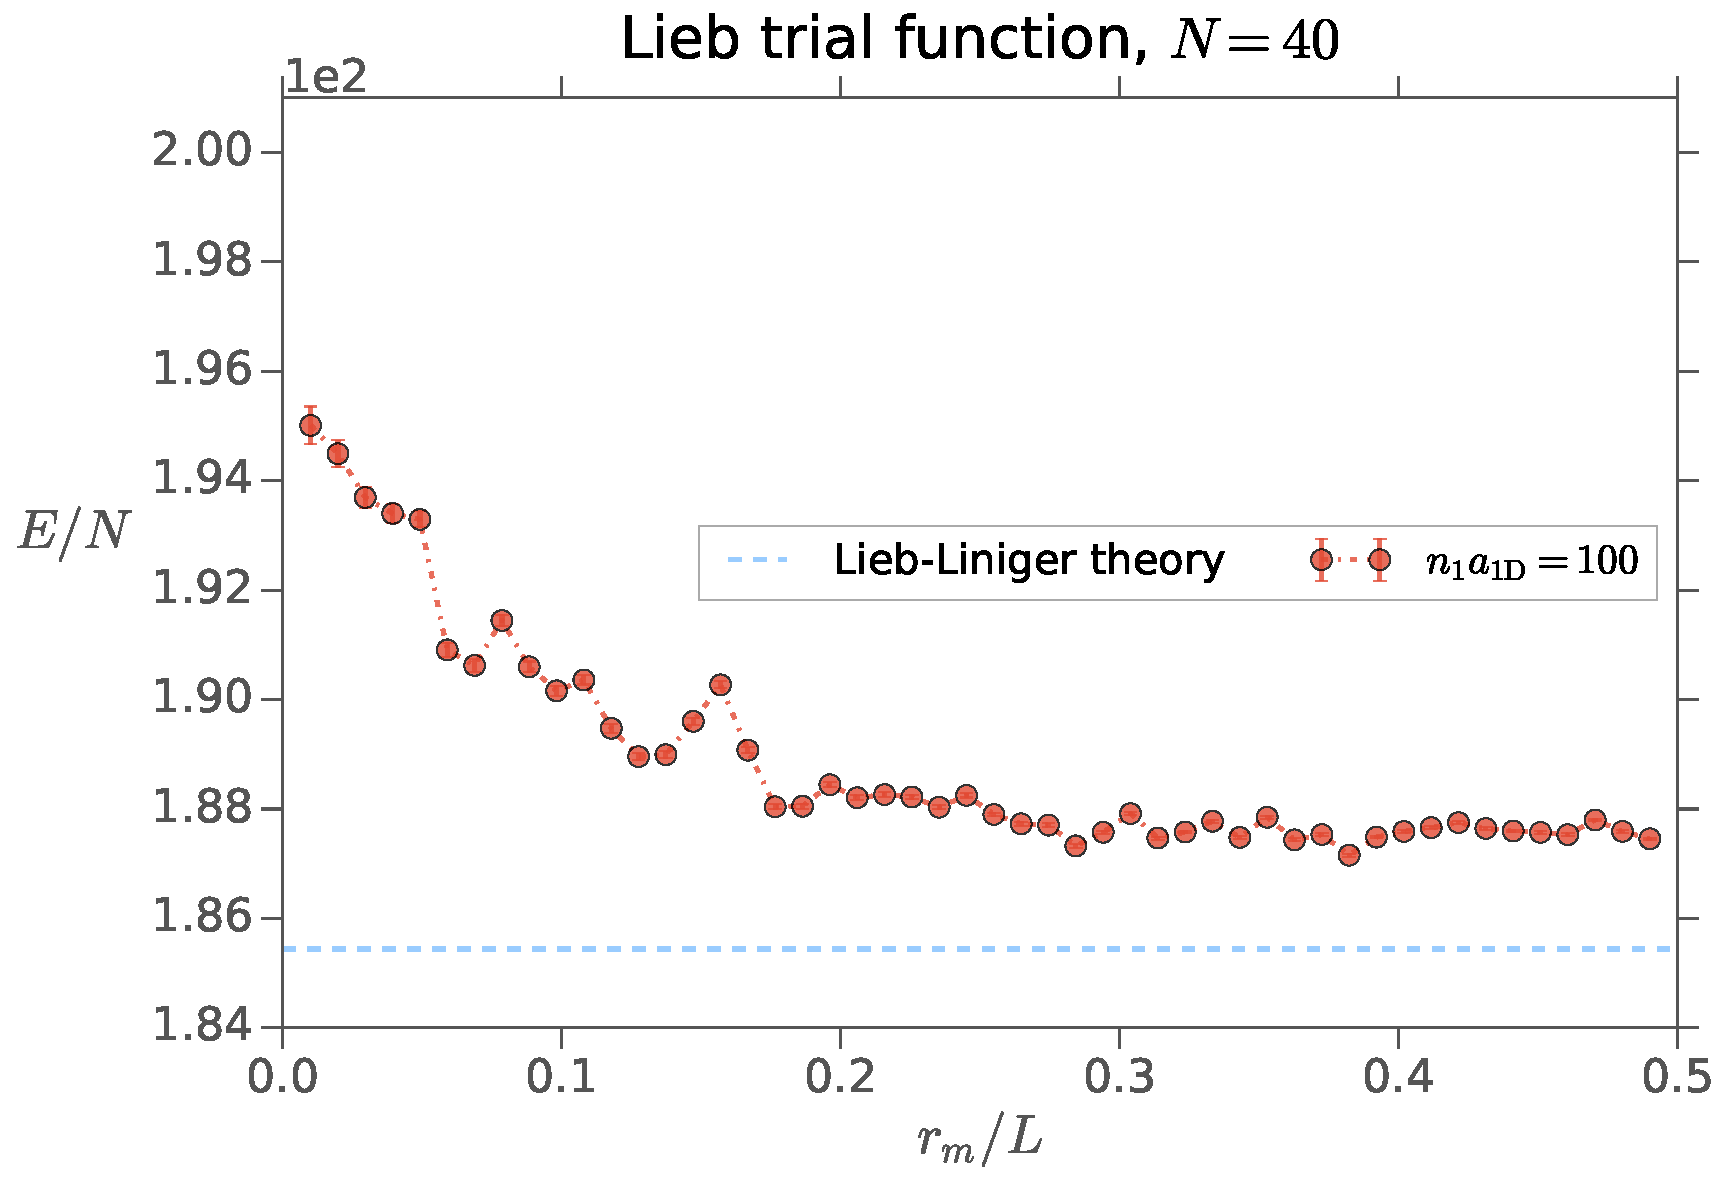
\includegraphics[width=0.75\linewidth]{./figures/lieb_energy-as-rm_n-a1d-100_Nb-40}
  \caption{Energy per boson (in units of $\hbar^2/2m\asonedim^2$) as a function
    of the variational parameter $r_m / L$ in the Gross-Pitaevskii regime. The
    energy decreases as the variational parameter grows, reaching a minimum (a
    plateau) after $r_m / L > 0.25$, and becoming independent of it. The energy
    predicted by the Lieb-Liniger theory has been added as a reference, showing
    that the variational energy is an upper bound to the exact energy. }
  \label{fig:lieb-energy-as-rm-n-a1d-100-nb-40}
\end{figure}
%
\begin{figure}[h!]
  \centering
  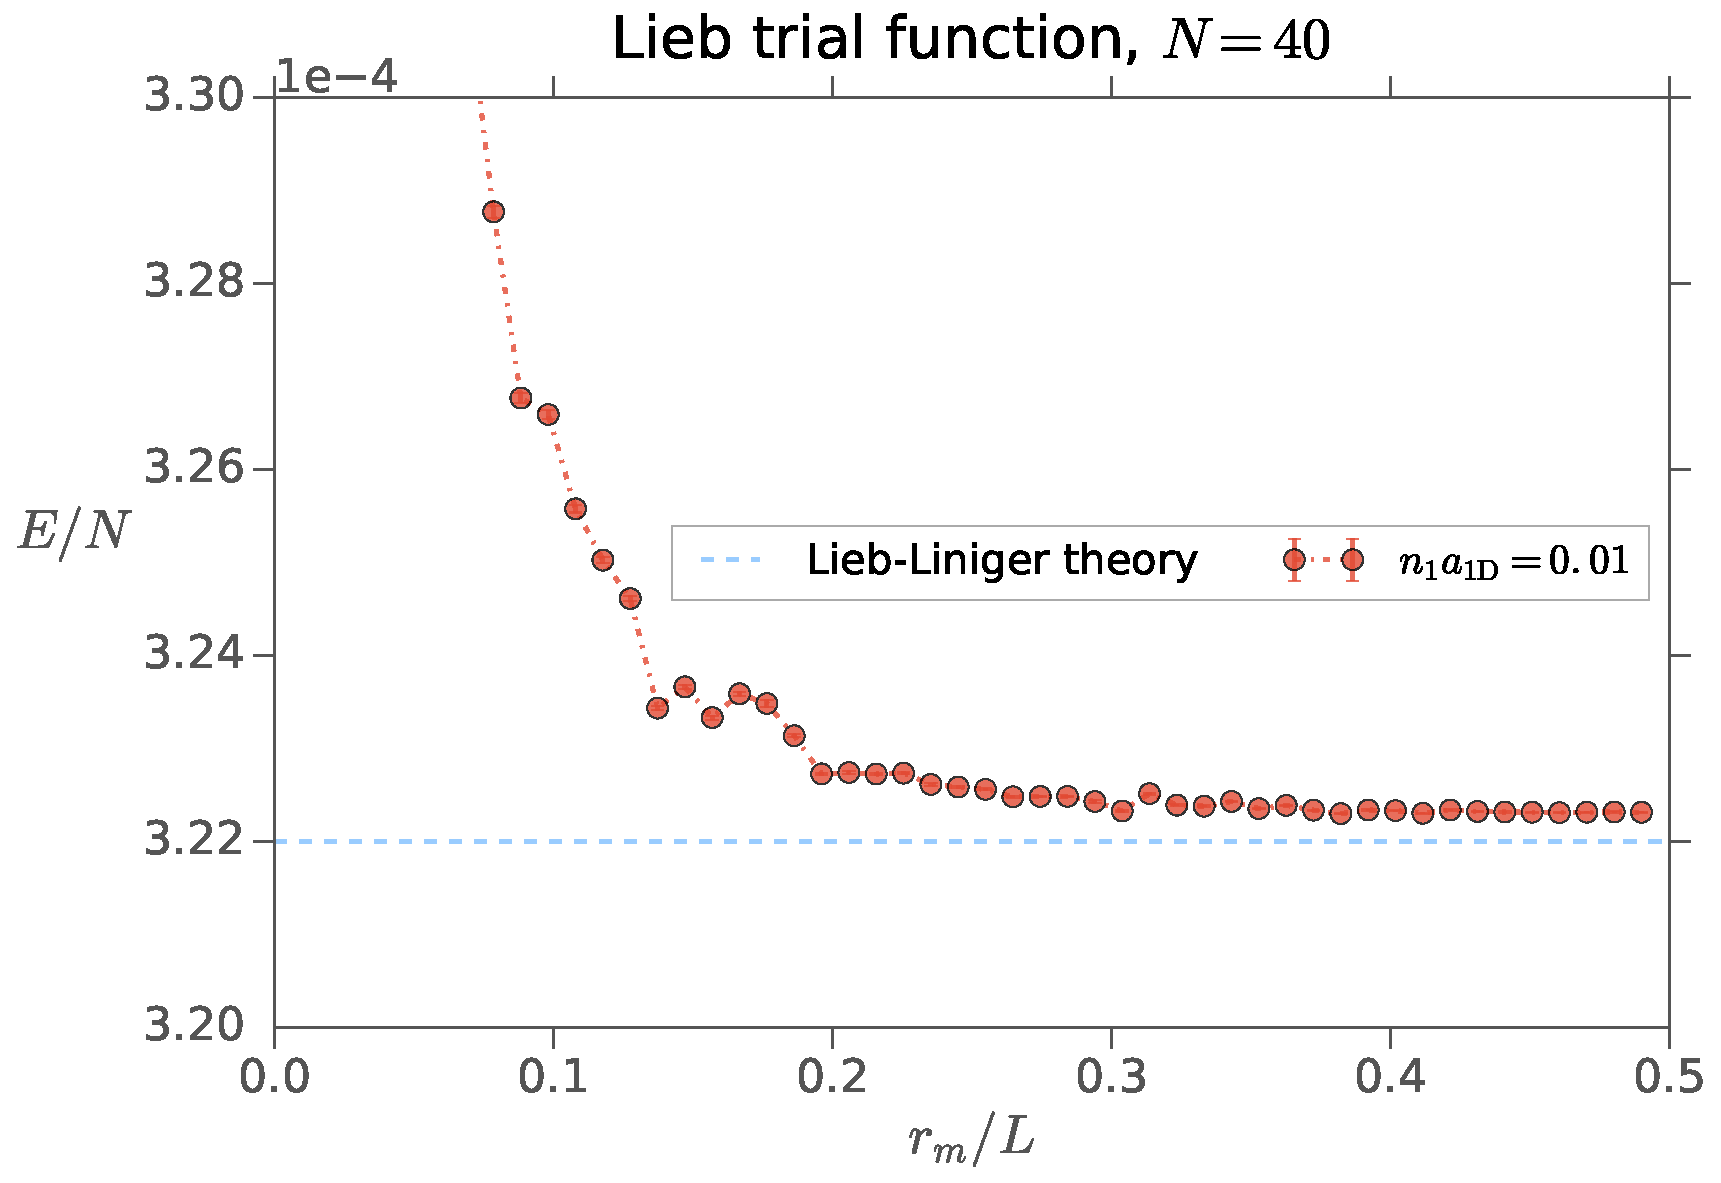
\includegraphics[width=0.75\linewidth]{./figures/lieb_energy-as-rm_n-a1d-0-dot-01_Nb-40}
  \caption{Energy per boson (in units of $\hbar^2/2m\asonedim^2$) as a function
    of the variational parameter $r_m / L$ in the Tonks-Girardeau regime. The
    energy decreases rapidly as the variational parameter grows, reaching a
    minimum (a plateau) after $r_m / L > 0.2$, effectively becoming independent
    of it. }
  \label{fig:lieb-energy-as-rm-n-a1d-0-dot-01-nb-40}
\end{figure}
%
\begin{figure}[t!]
  \centering
  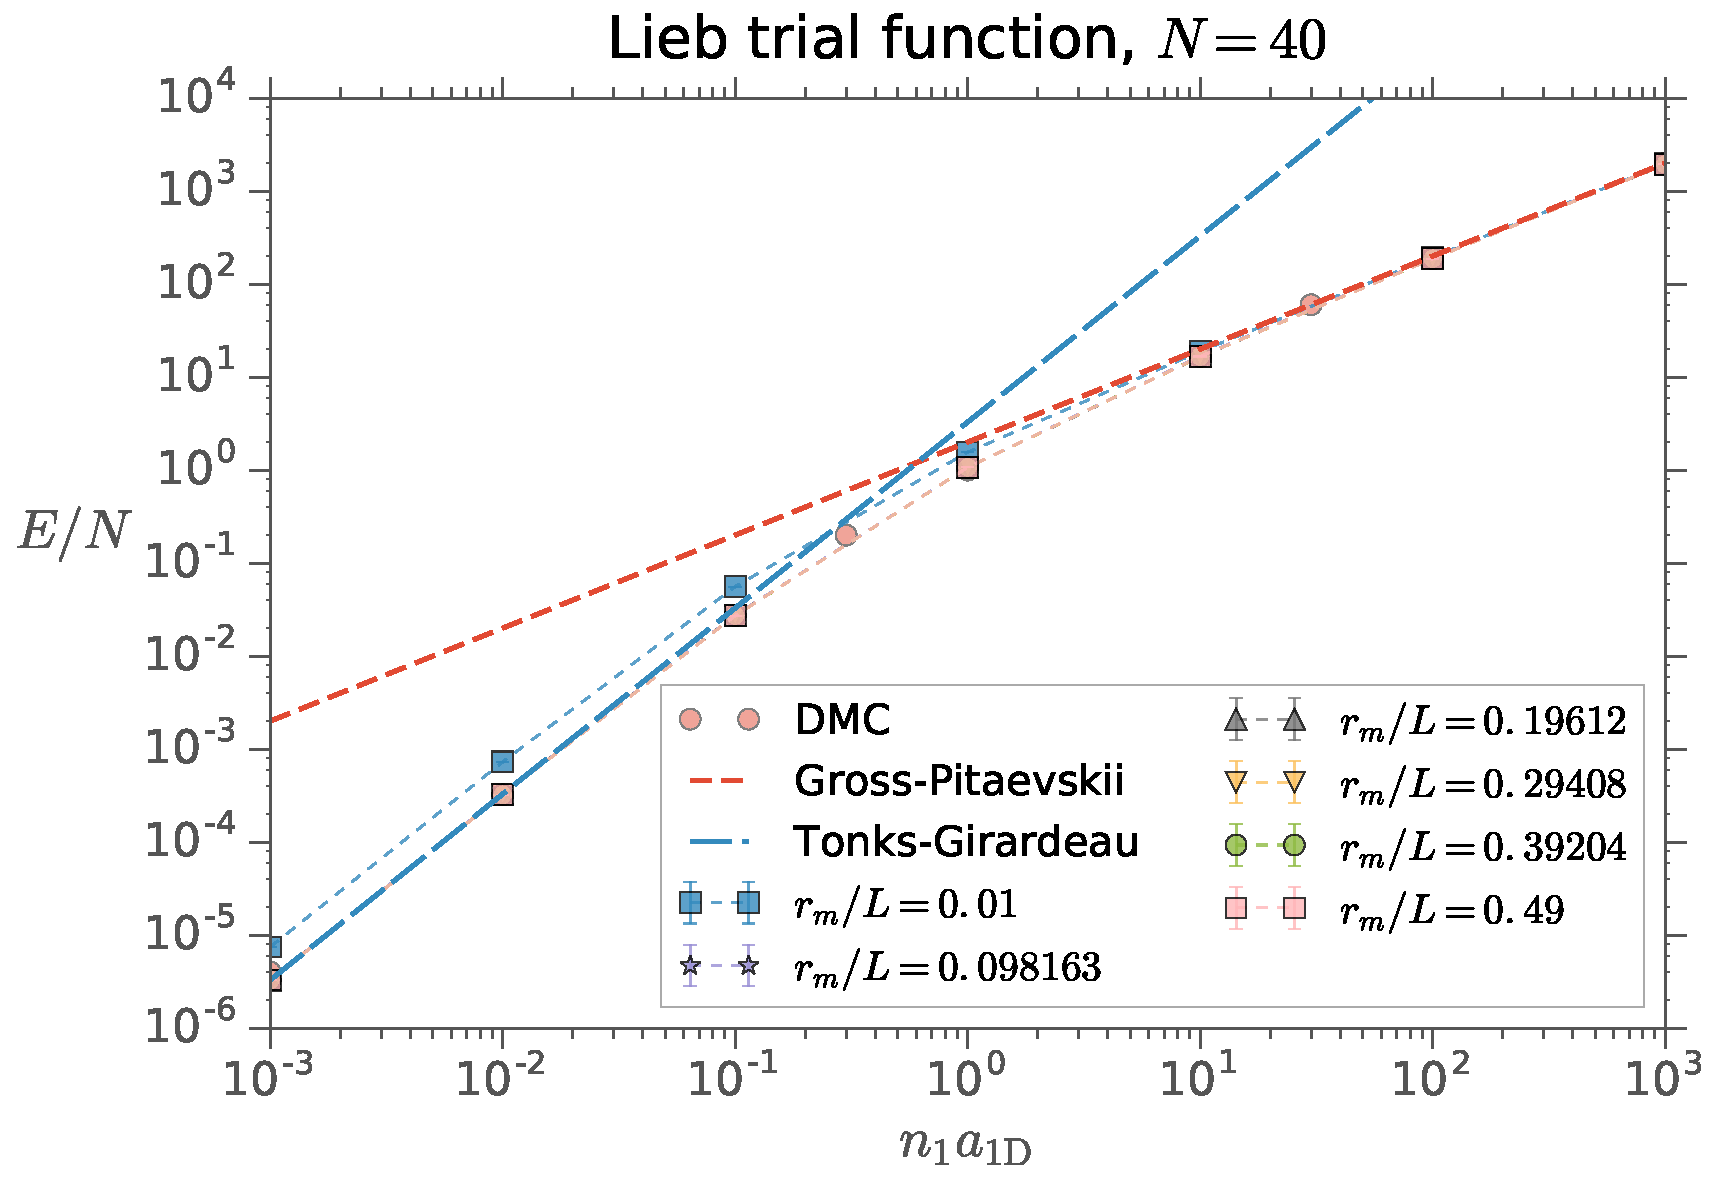
\includegraphics[width=0.75\linewidth]{./figures/lieb_energy-as-n-a1d_rm-var_Nb-40}
  \caption{Energy per boson (in units of $\hbar^2/2m\asonedim^2$) as a function
    of the gas parameter $\densityone \asonedim$ for several values of the
    variational parameter using a Lieb type trial function.  Some markers
    overlap and are not readily visible due to the small differences between the
    results. Markers with 	legend {DMC}, source:
    \cite{bib:astrakharchik-phys-rev-a.68.031602.2003}. }
  \label{fig:lieb-energy-as-n-a1d-rm-var-nb-40}
\end{figure}
%
The contribution to the local energy of the system of a pair of bosons and the
$j$-nth component of drift force are, respectively,
%
\begin{align}
  K_{\mathrm{L}}^2(r) & = \begin{cases}
    k_2^2 \, [1 + \tan^2(k_2(|r| - |r_m|))] & 0 \leq |r| < |r_m| \\
    0                                       & |r| > |r_m|
  \end{cases}  \\
  R_{j}(\vec z)       & = \begin{cases}
    -k_2 \displaystyle \sum_{\substack{k=1 \\ k \neq j}}^{N} \tan(k_2(|r_{kj}| - |r_m|)) \cdot \frac{z_j - z_k}{|z_j - z_k|} & 0 \leq |r| < |r_m| \\
    0 & |r| > |r_m|
  \end{cases}.
\end{align}
%

The results for the energy of the ground state are shown in the figures
\ref{fig:lieb-energy-as-rm-n-a1d-100-nb-40} and
\ref{fig:lieb-energy-as-rm-n-a1d-0-dot-01-nb-40} for the Gross-Pitaevskii and
the Tonks-Girardeau regimes respectively. In both cases the variational energy
decreases as the variational parameter $r_m / L$ increases, but rapidly reaches
a plateau and the energy becomes effectively independent of the variational
parameter beyond $r_m / L > 0.25$ approximately.

A global picture of the energy per boson is shown in the figure
\ref{fig:lieb-energy-as-n-a1d-rm-var-nb-40}, where the energy is shown as a
function of the gas parameter $\densityone \asonedim$ ranging from $10^{-3}$
(Tonks-Girardeau) up to $10^{3}$ (Gross-Pitaevskii). The results from {VMC} were
calculated for several values of $r_m / L$ in order to show the dependence on
the variational parameter. The variational results are plotted along with the
curves for the Gross-Pitaevskii and the Tonks-Girardeau approximation, and with
the results obtained through DMC
\cite{bib:astrakharchik-phys-rev-a.68.031602.2003}.

In general we can see that the Lieb two-body trial function is a good enough
choice to obtain results within five percent of relative error with respect to
the exact results.
%

\subsection{Phonon trial function}

The Phonon trial function is defined in such way that is a solution of the
two-body Schrödinger equation for a delta interaction potential at short
distances $0 < |r| < |r_m|$, and for $|r| > |r_m|$ it arises from a phononic
behavior \cite[]{bib:reatto-phys-rev.155.1967} . The exact definition of the
two-body function is
%
\begin{equation}
  \label{eq:vmc-phonon-two-body-function}
  f_2(r) = \begin{cases}
    A \cos(k_2(|r| - r_0))                      & 0 \leq|r| < |r_m| \\
    \sin^{\beta}\left(\frac{\pi |r|}{L} \right) & |r| > |r_m|
  \end{cases},
\end{equation}
%
with $r$ the relative distance between two bosons and $r_m$ being the
variational parameter, as with the Lieb trial function. The parameter $r_0$ is
an offset used to join both parts of the functions. For $r = L/2$ the wave
function is equal to one, i.e., the two bosons become uncorrelated. In general,
any trial wave function must have that property.

In order to determine then coefficients we impose the following boundary
conditions on the function:
%
\begin{itemize}
  \item At the origin it satisfies the relation $k_2 \asonedim \tan(k_2 r_0) =
          1$ because of the delta interaction between the bosons.

  \item It must be continuous a the matching point $r_m$, so
        %
        \begin{equation}
          A \cos(k_2(|r_m| - r_0)) = \sin^{\beta}\left(\frac{\pi |r_m|}{L} \right).
        \end{equation}

  \item Its derivative must be continuous at $r_m$. This condition, together
        with the continuity of $f_2$ yields the next equality:
        %
        \begin{equation}
          -k_2 \tan(k_2(|r_m| - r_0)) = \frac{\pi}{L} \beta \cot\left(\frac{\pi |r_m|}{L} \right).
        \end{equation}

  \item The local energy must be continuous at $r_m$. Together with the two
        previous conditions this one yields
        %
        \begin{equation}
          -k_2^2 = \left(\frac{\pi}{L}\right)^2 \beta \left[ (\beta - 1) \cot^2\left(\frac{\pi |r_m|}{L} \right) -1 \right]
        \end{equation}
\end{itemize}
%
We solve this system of equations and we can find the four parameters $k_2$,
$r_0$, $\beta$ and $A$. Once we know these values we can evaluate the local
energy. The contribution of the bosons to the local energy is
%
\begin{equation}
  K_{\mathrm{L}}^2(r) = \begin{cases}
    k_2^2 \, [1 + \tan^2(k_2(|r| - r_0))]                                                       & 0 \leq |r| < |r_m| \\
    \left(\frac{\pi}{L}\right)^2 \beta \left[ 1 + \cot^2\left(\frac{\pi |r|}{L} \right) \right] & |r| > |r_m|
  \end{cases},
\end{equation}
%
while the contribution to the $j$-nth component of the drift force is
%
\begin{equation}
  R_{j}(\vec z) = \begin{cases}
    -k_2 \displaystyle \sum_{\substack{k=1                                  \\ k \neq j}}^{N} \tan(k_2(|r_{kj}| - r_0)) \cdot \frac{z_j - z_k}{|z_j - z_k|} & 0 \leq |r| < |r_m| \\
    \frac{\pi}{L} \beta \cot \left( \frac{\pi |r|}{L} \right) & |r| > |r_m|
  \end{cases}.
\end{equation}
%
The energy as a function of the variational parameter $r_m / L$ is shown in the
figures \ref{fig:phonon-energy-as-rm-n-a1d-100-nb-40} and
\ref{fig:phonon-energy-as-rm-n-a1d-0-dot-01-nb-40}. The results show a very
similar behavior as in the case of the Lieb trial function, as the energy
decreases as $r_m / L$ increases. However, the value of the energy for the
Phonon trial function remains constant during a greater interval of the
variational parameter, specially in the Tonks-Girardeau regime ($\densityone
  \asonedim \ll 1$). This suggests that the Phonon trial function is a better
two-body function to model the behavior of the interaction between the bosons.
%
\begin{figure}[h!]
  \centering
  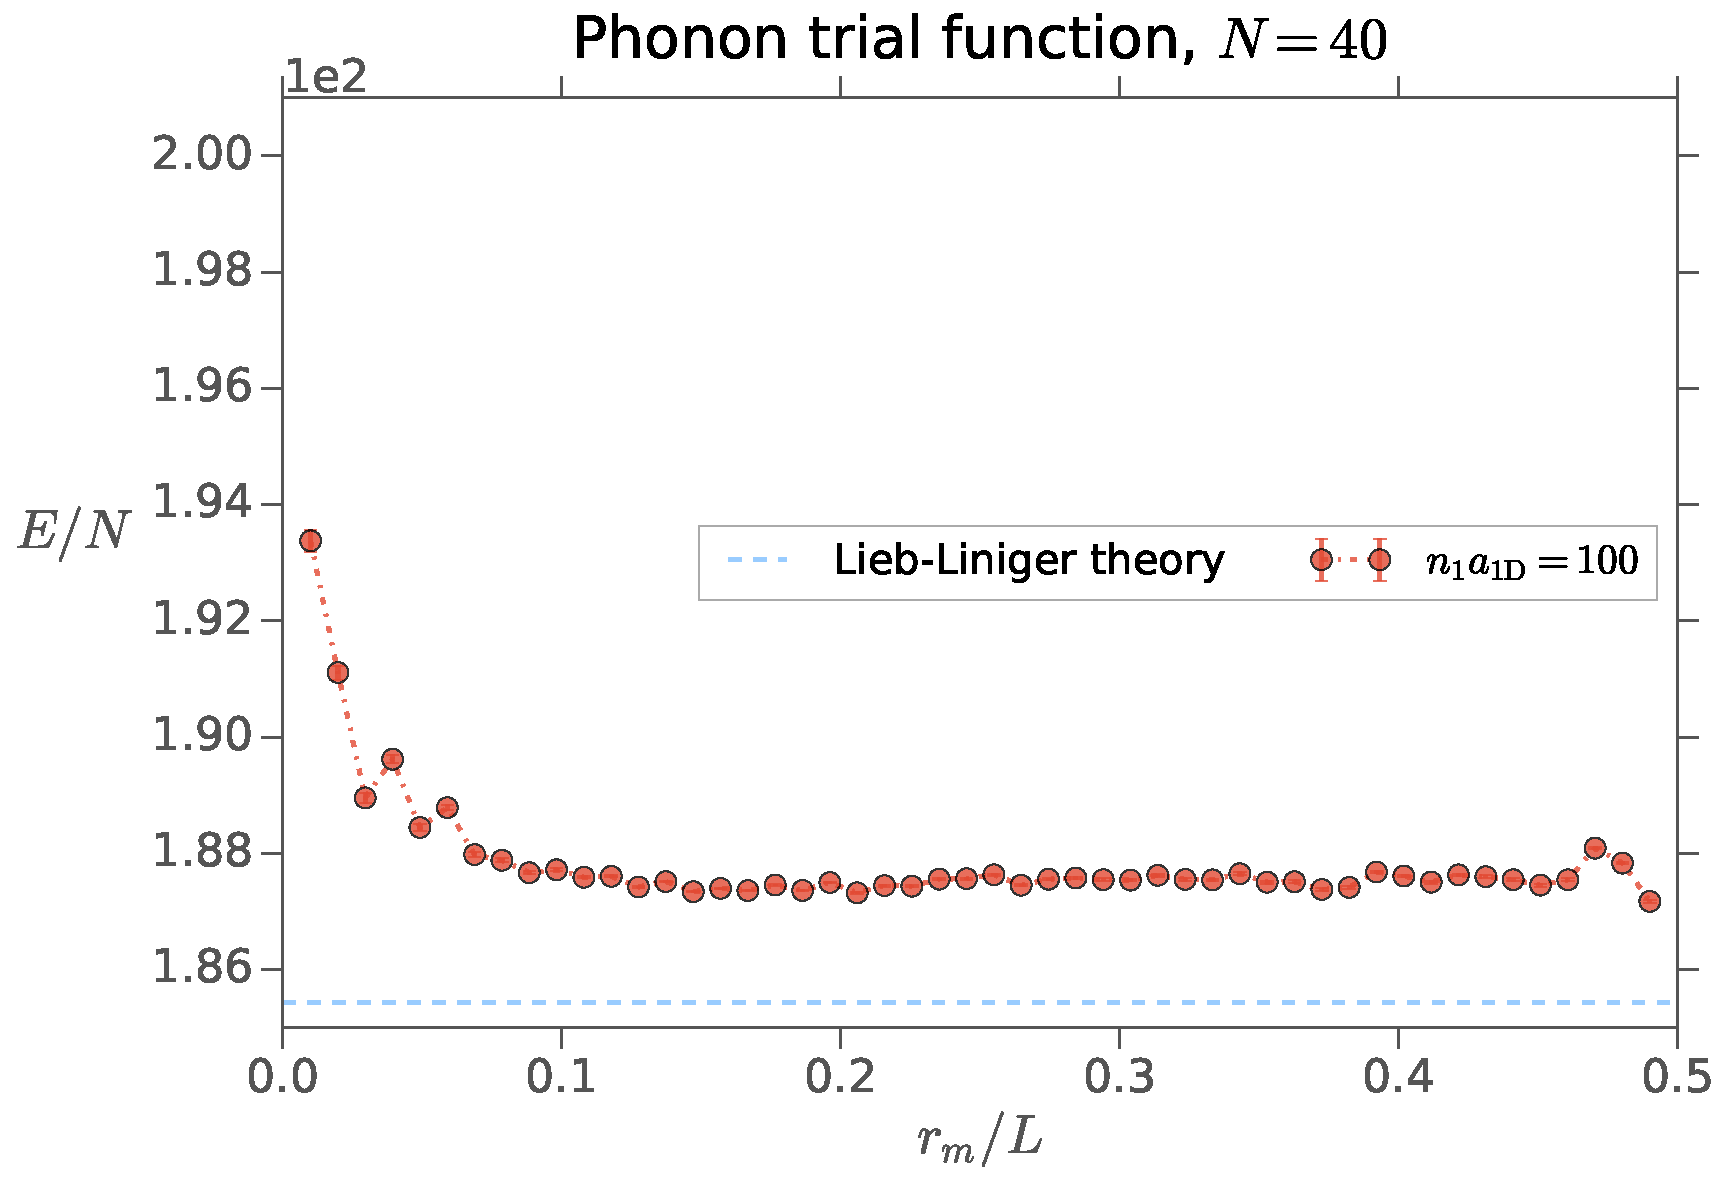
\includegraphics[width=0.75\linewidth]{./figures/phonon_energy-as-rm_n-a1d-100_Nb-40}
  \caption{ Energy per boson (in units of $\hbar^2/2m\asonedim^2$) as a function
    of the variational parameter $r_m / L$ in the Gross-Pitaevskii regime. }
  \label{fig:phonon-energy-as-rm-n-a1d-100-nb-40}
\end{figure}
%
\begin{figure}[h!]

  \centering
  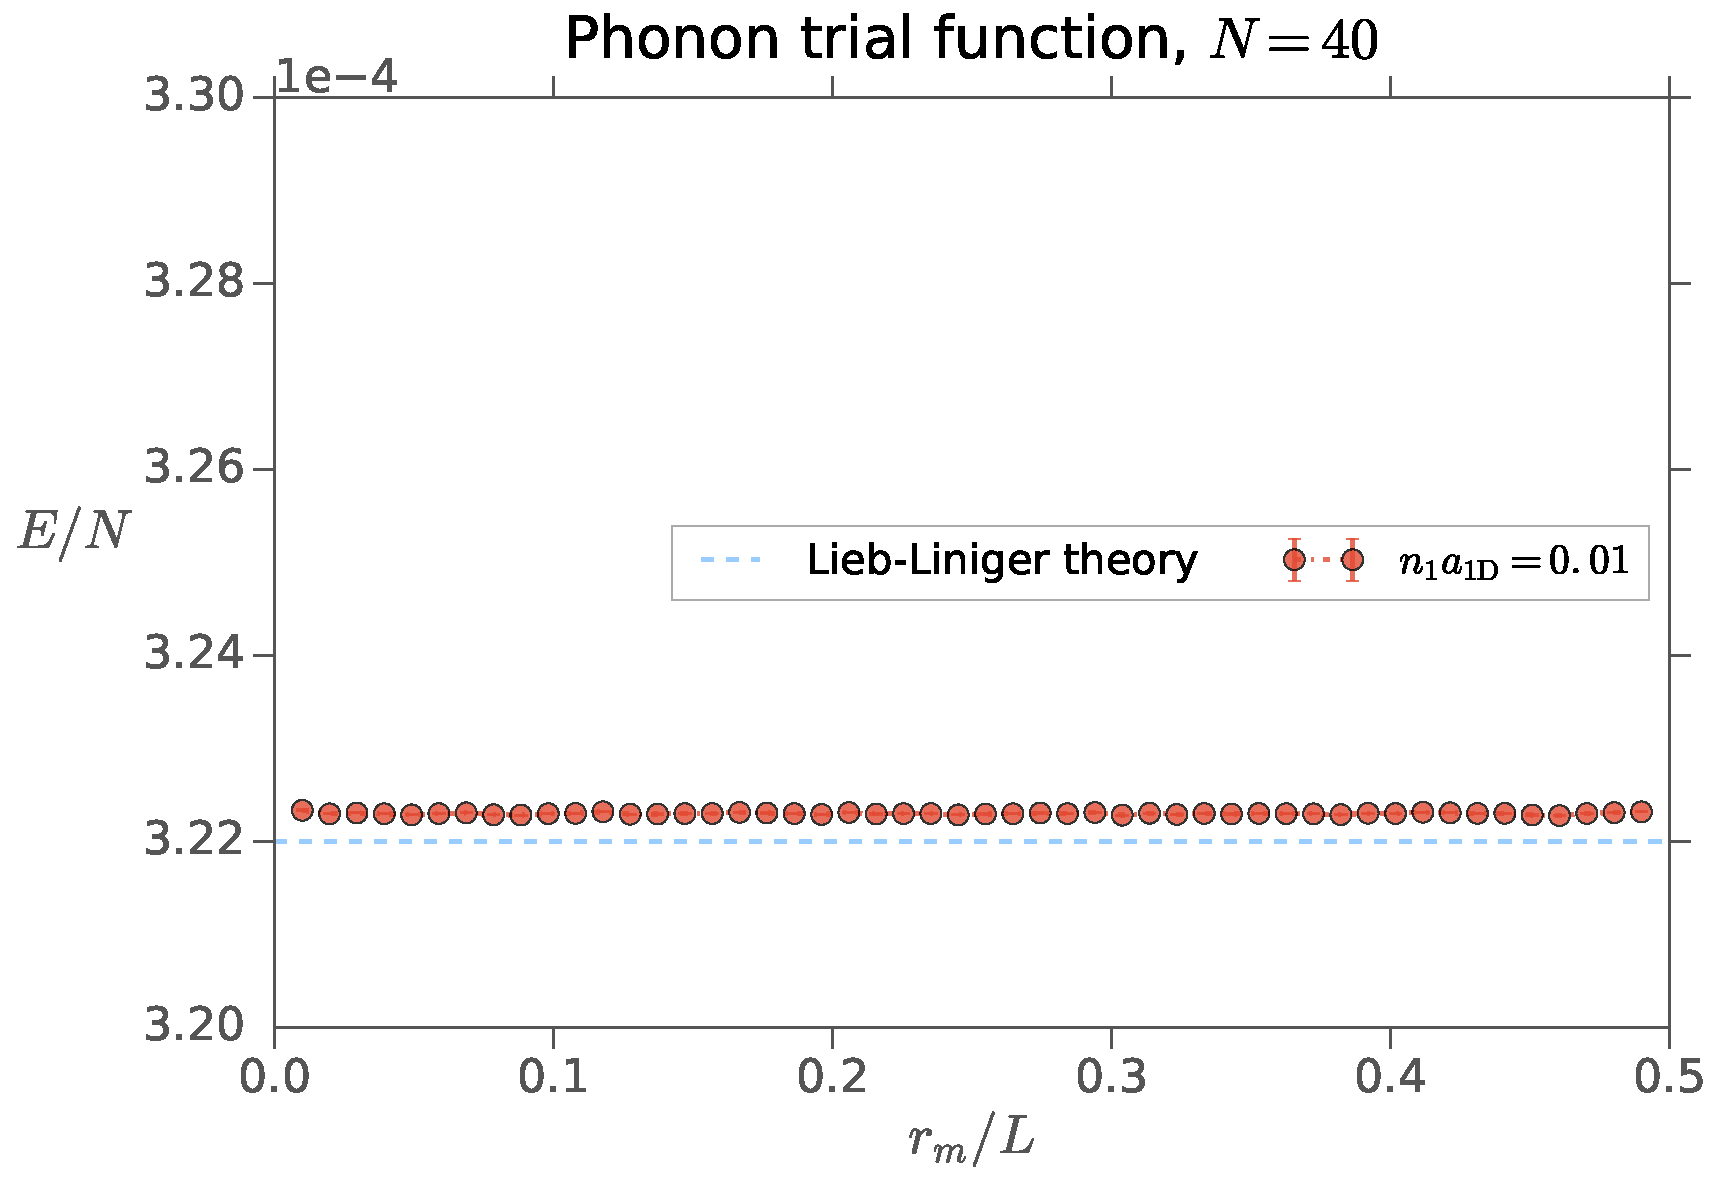
\includegraphics[width=0.75\linewidth]{./figures/phonon_energy-as-rm_n-a1d-0-dot-01_Nb-40}
  \caption{ Energy per boson (in units of $\hbar^2/2m\asonedim^2$) as a function
    of the variational parameter $r_m / L$ in the Tonks-Girardeau regime. }
  \label{fig:phonon-energy-as-rm-n-a1d-0-dot-01-nb-40}
\end{figure}
%
\begin{figure}[h!]
  \centering
  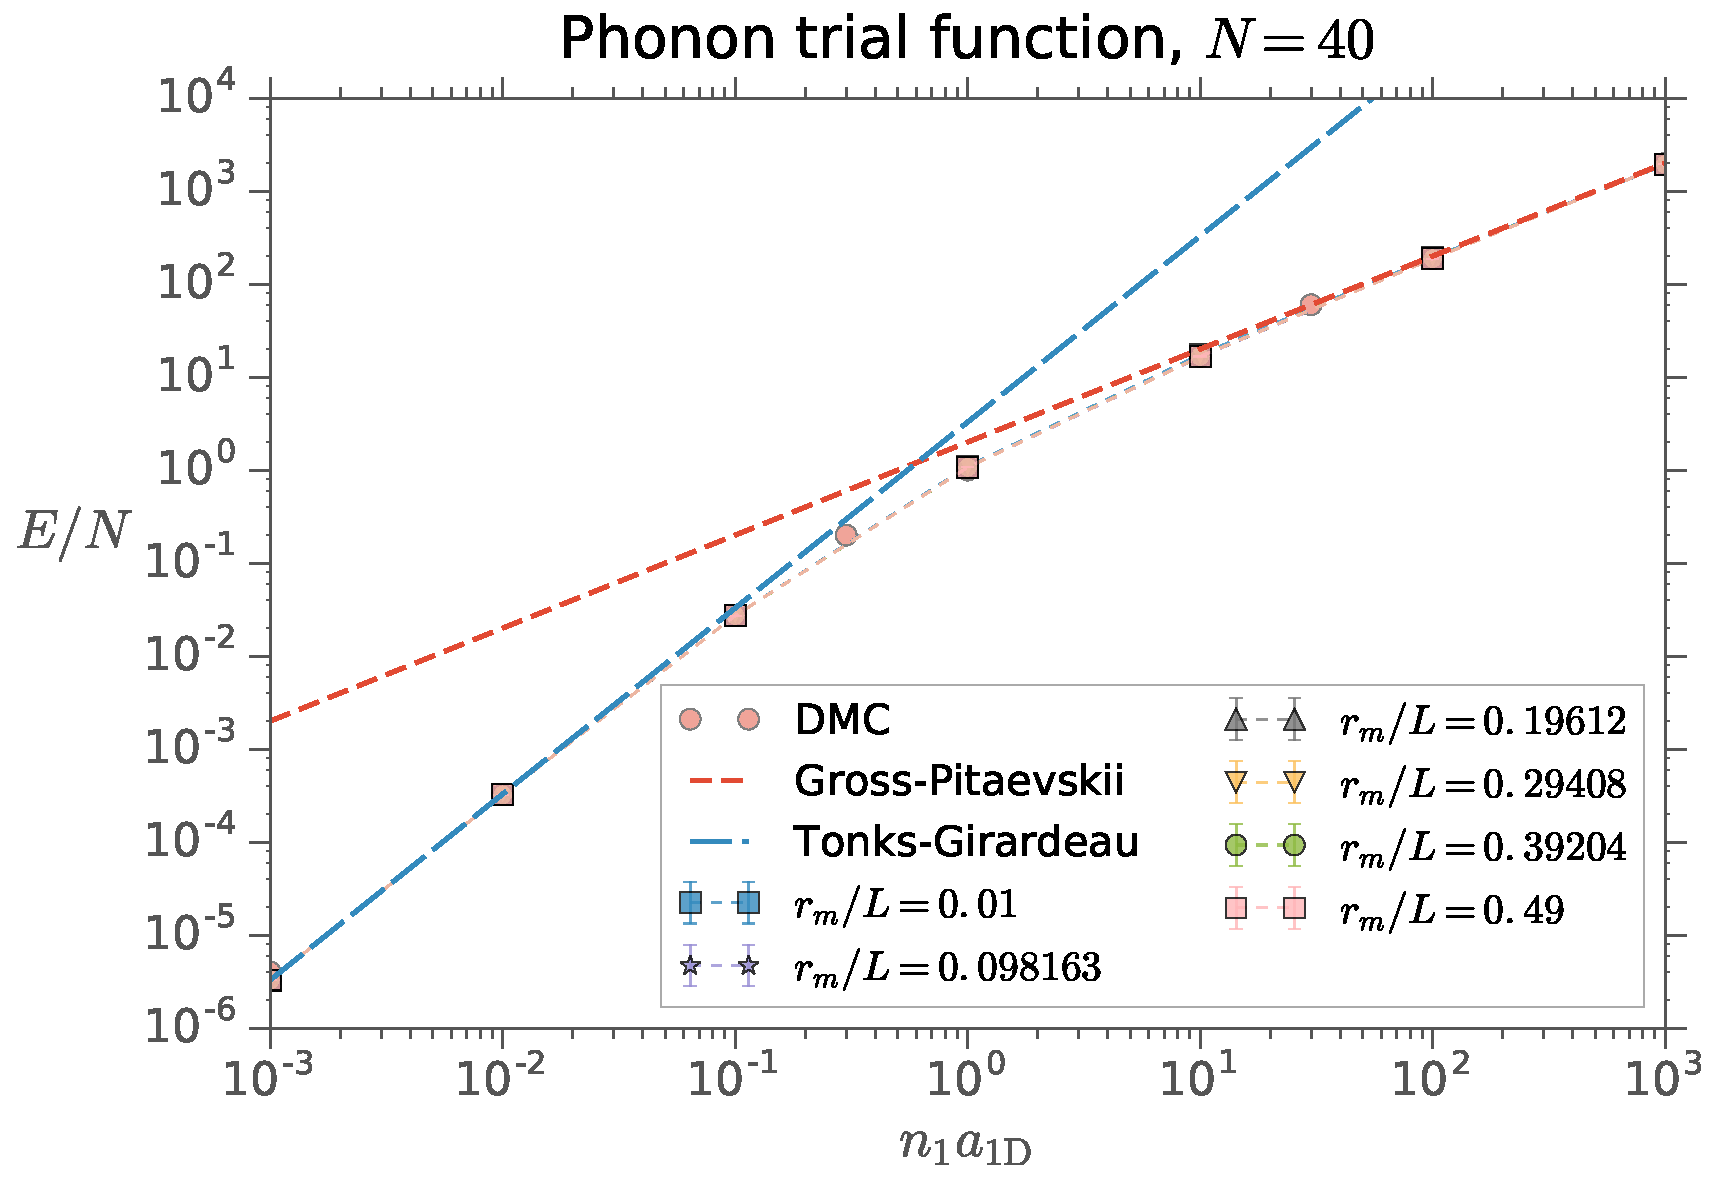
\includegraphics[width=0.75\linewidth]{./figures/phonon_energy-as-n-a1d_rm-var_Nb-40}
  \caption{ Energy per boson in units of $\hbar^2 / 2 m \asonedim^2$ of the
    Lieb-Liniger gas calculated using VMC with forty particles using a Phonon
    type trial function for several values of the variational parameter $r_m /
      L$. }
  \label{fig:phonon-energy-as-n-a1d-rm-var-nb-40}
\end{figure}



\subsection{Comparison of trial functions}

The comparison of the Lieb and Phonon trial functions, plotted in fig.
\ref{fig:comparison-energy-as-n-a1d-nb-40} makes evident a great similarity in
the results for the energy per boson when the value of the variational parameter
is $r_m / L = 0.2451$. This value was chosen because, accordingly to our
previous discussion about the behavior of the energy as a function of $r_m$, it
is a good value that minimizes the energy per boson.
%
\begin{figure}[h!]
  \centering
  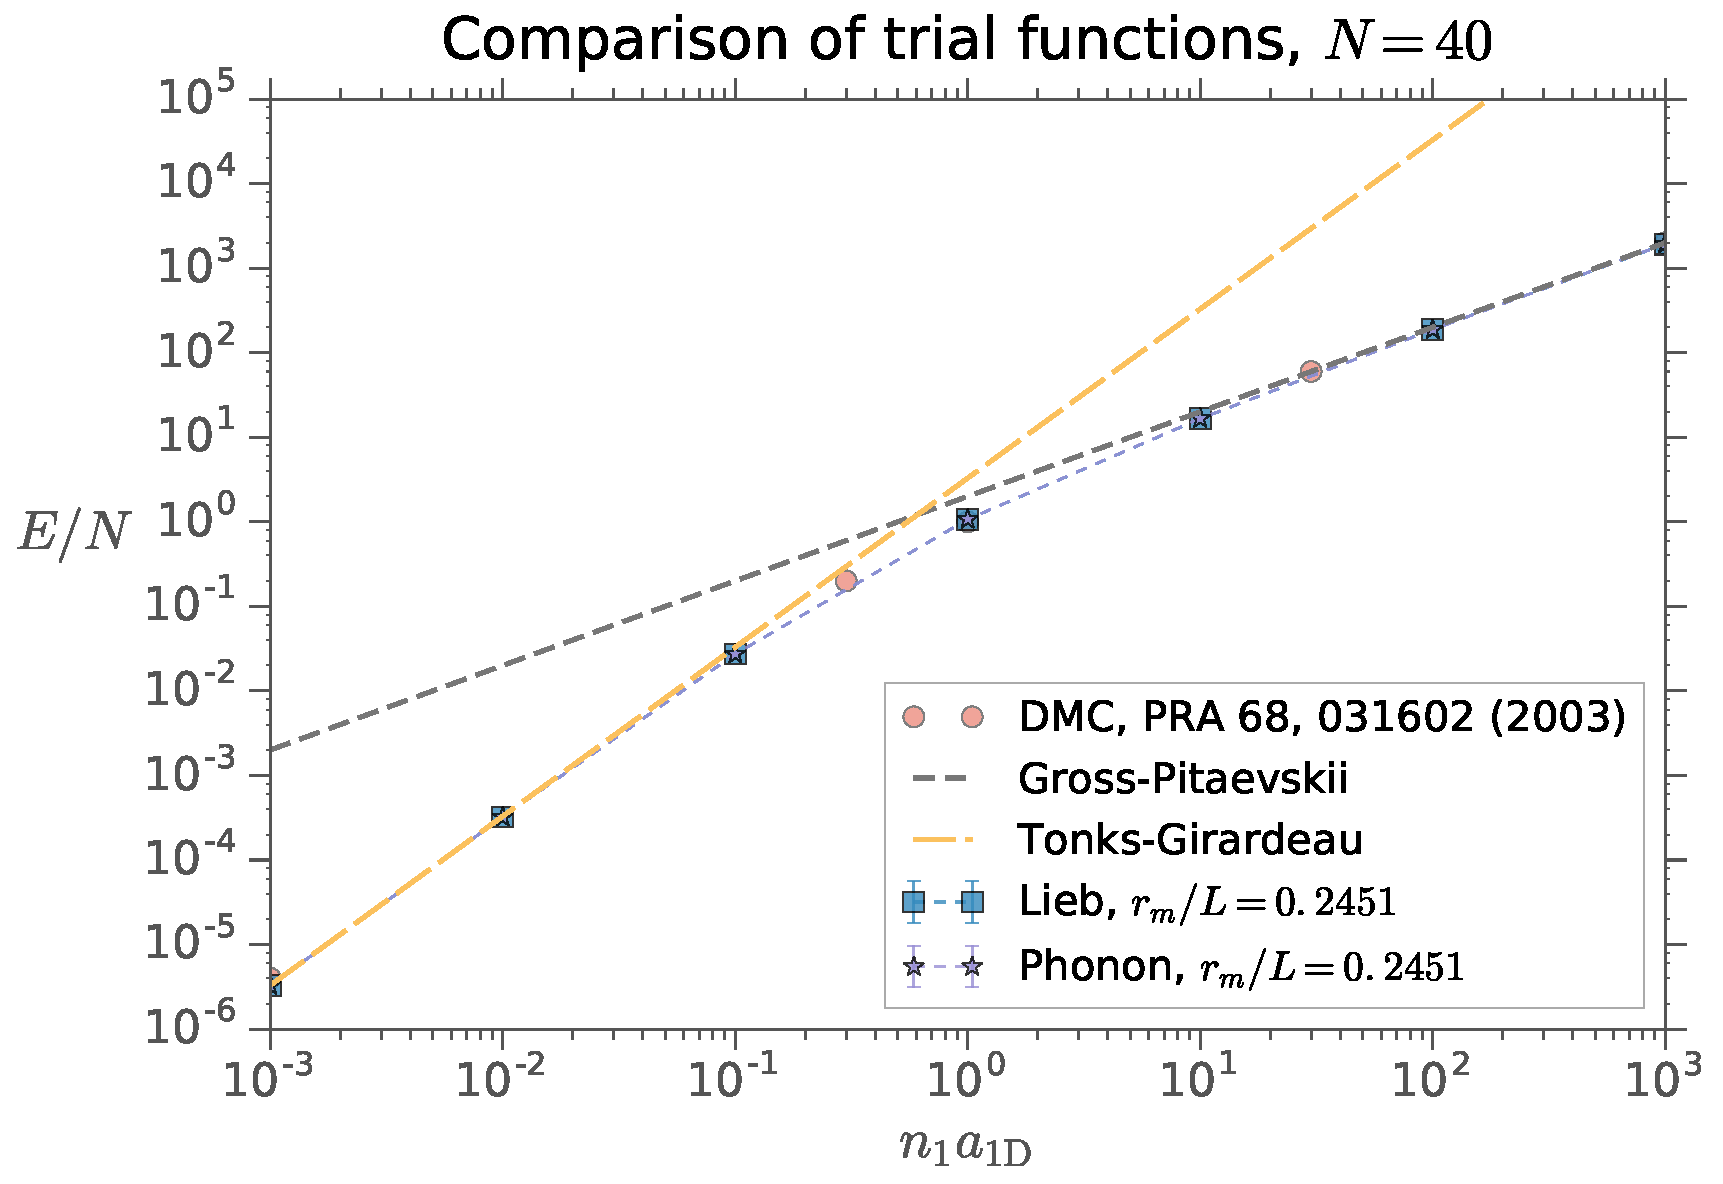
\includegraphics[width=0.75\linewidth]{./figures/comparison_energy-as-n-a1d_Nb-40}
  \caption{ Comparison of the energy per boson (in units of $\hbar^2 / 2 m
      \asonedim^2$) calculated with VMC using the Lieb trial function (square
    markers) and the Phonon trial function (star markers) along with the results
    calculated with DMC \cite{bib:astrakharchik-phys-rev-a.68.031602.2003}. }
  \label{fig:comparison-energy-as-n-a1d-nb-40}
\end{figure}
%
The results in figure \ref{fig:comparison-energy-as-n-a1d-nb-40} effectively
show that both trial functions are as good as the other, and the energies
calculated are very close to the predicted by DMC and Lieb-Liniger theory.

The results  lead us to choose the Phonon trial function to model the
interactions between the bosons for the Bose gas within the Kronig-Penney
potential.



\subsection{VMC for a gas within a multi-rods potential}

We realized VMC for a Bose gas within a Kronig-Penney external potential using
the phonon two-body functions \eqref{eq:vmc-phonon-two-body-function} as before,
in addition to the one-body functions
%
\begin{align}
  f_1(z) = \begin{cases}
    \cos \left[k_1 \left(z - jl - \frac{a}{2} \right)\right]         & j(a + b) < z < j(a+b) + a       \\
    A \cosh\left[\kappa_1 \left(z - jl + \frac{b}{2} \right) \right] & j(a + b) + a < z < (j+1)(a + b)
  \end{cases},
\end{align}
%
where $l = a + b$ is the period of the potential, $j$ is an integer ranging from
minus infinity to infinity, $\hbar k_1 = \sqrt{2m\ez[0]}$ and $\hbar \kappa_1 =
  \sqrt{2m(V_0 - \ez[0])}$. This function is a particular solution for the ground
state of Schrödinger equation for one particle subject to a Kronig-Penney
potential (see section
\ref{sec:the-ideal-bose-gas-within-a-kronig-penney-potential}). The parameter
$\ez[0]$ is the ground state energy and is fixed by eq.
\eqref{eq:kronig-penney-energy} with $\kz = 0$. The definition of $f_1(z)$ has
two parts: the \textit{cosine} part corresponds to the region where there is no
external potential, while the \textit{hyperbolic cosine} part does to the region
where $V_\mathrm{ext}(z) = V_0$. The constant $A$ is fixed by requiring
continuity of the derivative of the function at the interfaces of the potential
barriers, but we do not impose the normalization condition on the function as is
not necessary. The constant A is given as
%
\begin{equation}
  A = \sqrt{1 + \frac{V_0}{\ez[0]} \sinh^2\left( \frac{\kappa_1 b}{2} \right)}.
\end{equation}

Some results for the estimation of the energy per boson of the system in the
fig. \ref{fig:phonon-energy-as-gamma-rm-var-Nb-40}, where we plotted the energy
as a function of the interaction parameter $\gamma$. We also show the energy
difference with respect to the Lieb-Liniger theory in figure
\ref{fig:phonon-relative-energy-as-gamma-rm-var-nb-40}. Here it is evident how
even in the case when no external potential is applied the VMC simulation yield
results which are somewhat different from those predicted by the exact theory.
%
\begin{figure}[h!]
  \centering
  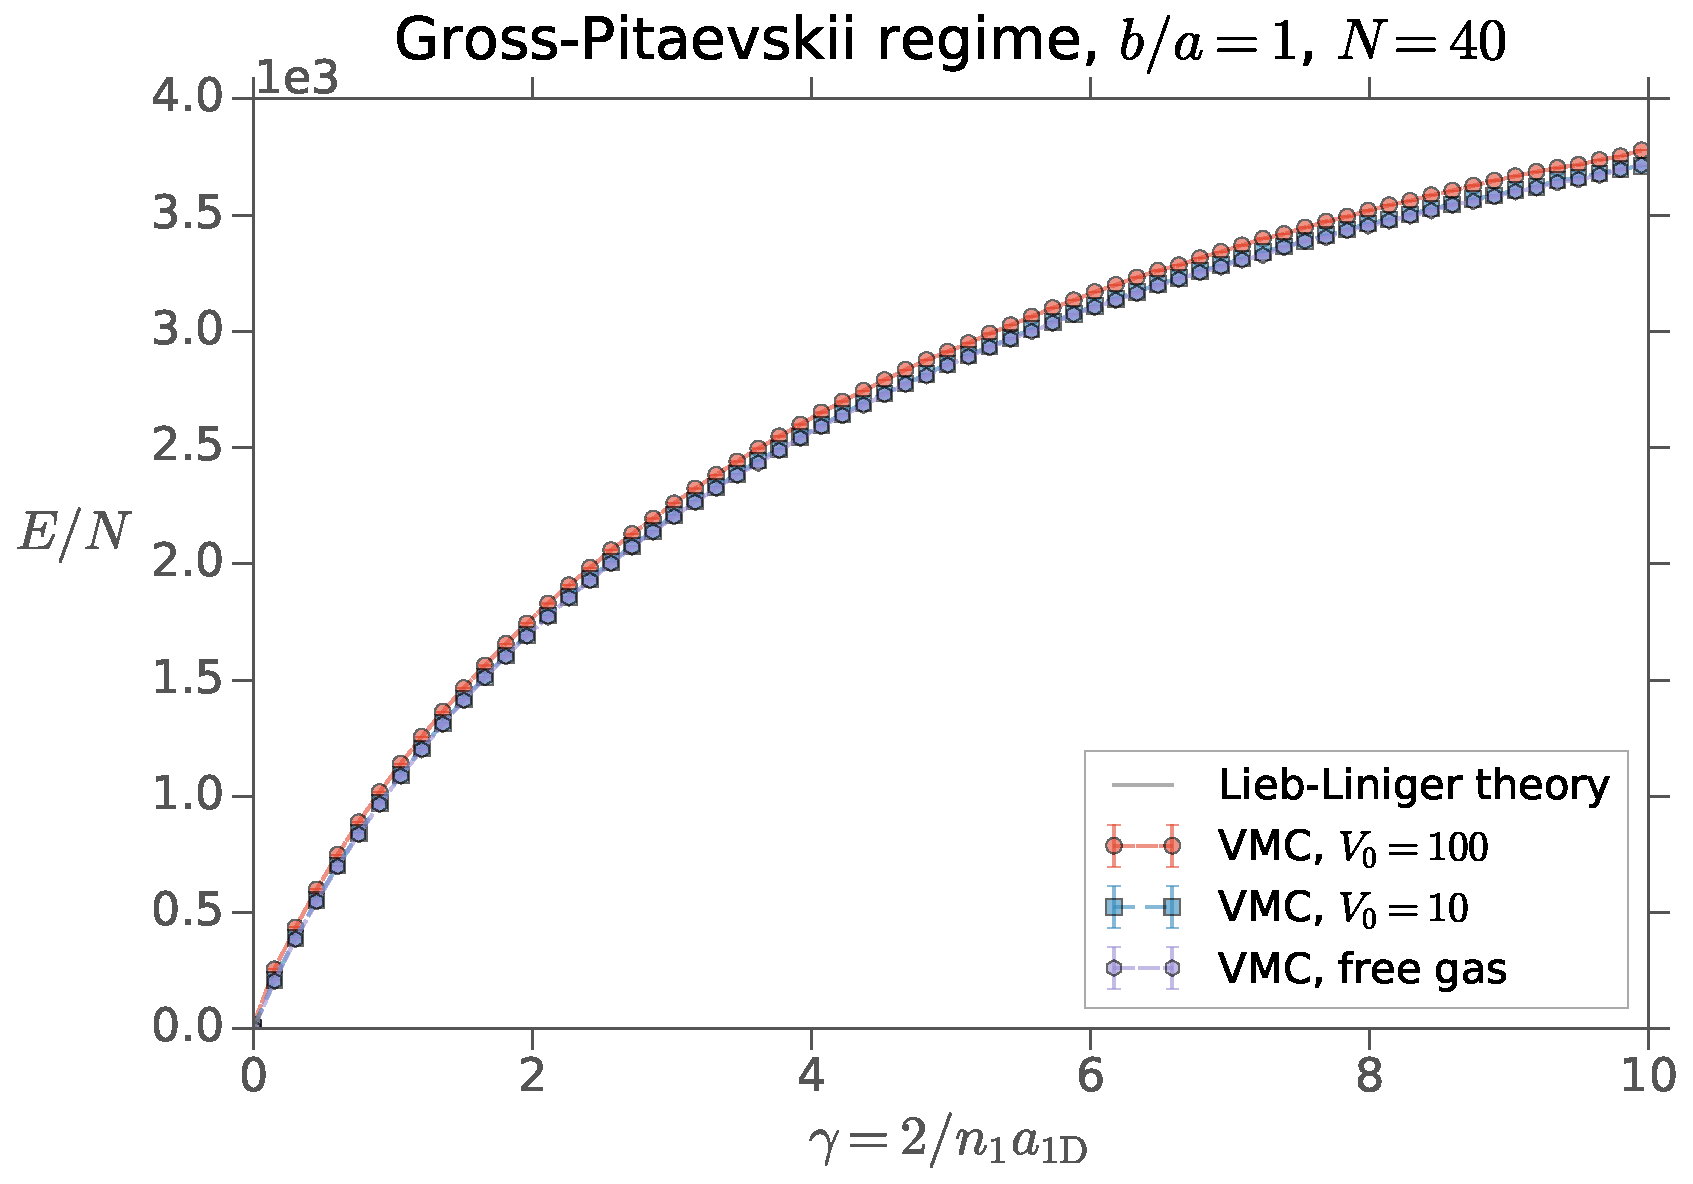
\includegraphics[width=0.75\linewidth]{./figures/phonon_energy-as-gamma_rm-var_Nb-40}
  \caption{ Comparison of the energy per boson $E/N$ (in units of $\hbar^2/2m(a
      + b)^2$) as a function of $\gamma$ calculated from the Lieb-Liniger theory
    \eqref{eq:lieb-liniger-energy} and through a VMC simulation with forty
    particles. We can see that the variational results for $V_\mathrm{ext} = 0$
    are slightly above to those predicted by the Lieb-Liniger theory. The
    statistical error of the approximation obtained from VMC is less than the
    size of the graph markers. }
  \label{fig:phonon-energy-as-gamma-rm-var-Nb-40}
\end{figure}
%
\begin{figure}
  \centering
  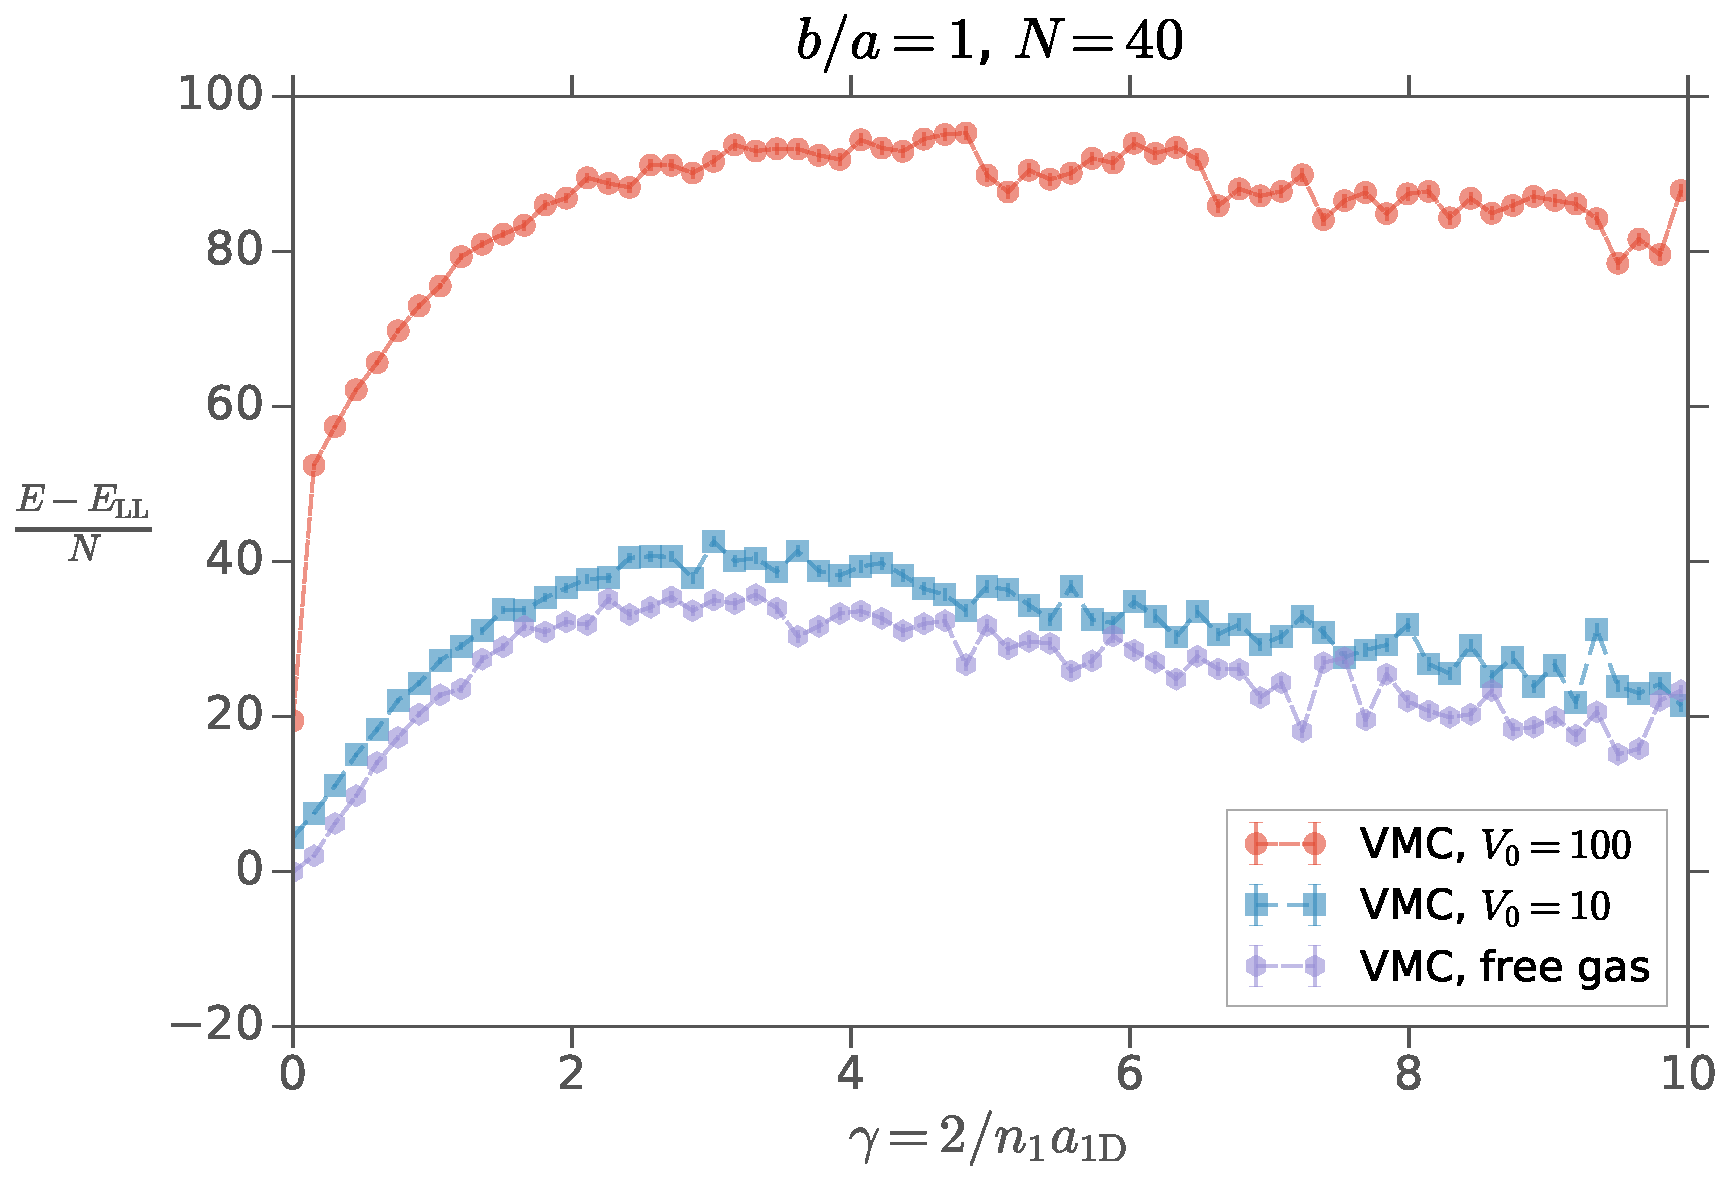
\includegraphics[width=0.75\linewidth]{./figures/phonon_relative-energy-as-gamma_rm-var_Nb-40}
  \caption{Energy per boson difference (in units of $\hbar^2/2m(a + b)^2$)
    between the VMC results and the energy predicted by the Lieb-Liniger
    theory.}
  \label{fig:phonon-relative-energy-as-gamma-rm-var-nb-40}
\end{figure}
%

In addition, we made a comparison of the energy per boson calculated both with
the Gross-Pitaevskii equation and Variational Monte Carlo in the mean-field
regime. To this end we realized calculations for small values of $\gamma$ in the
same interval as those results presented in fig.
\ref{fig:gross-pitaevskii-energy-as-gamma-nb-40}. The results are plotted in
fig. \ref{fig:phonon-gp-energy-as-gamma-rm-var-nb-40}. Variational and
mean-field energies have very similar values, although the second are slightly
greater. Accordingly with fig. \ref{fig:phonon-energy-as-gamma-rm-var-Nb-40} as
$\gamma$ grows is expected that these difference will increase and the
mean-field results will diverge from the variational ones. However, for small
values of $\gamma$ we consider that the results are very satisfactory.


\begin{figure}
  \centering
  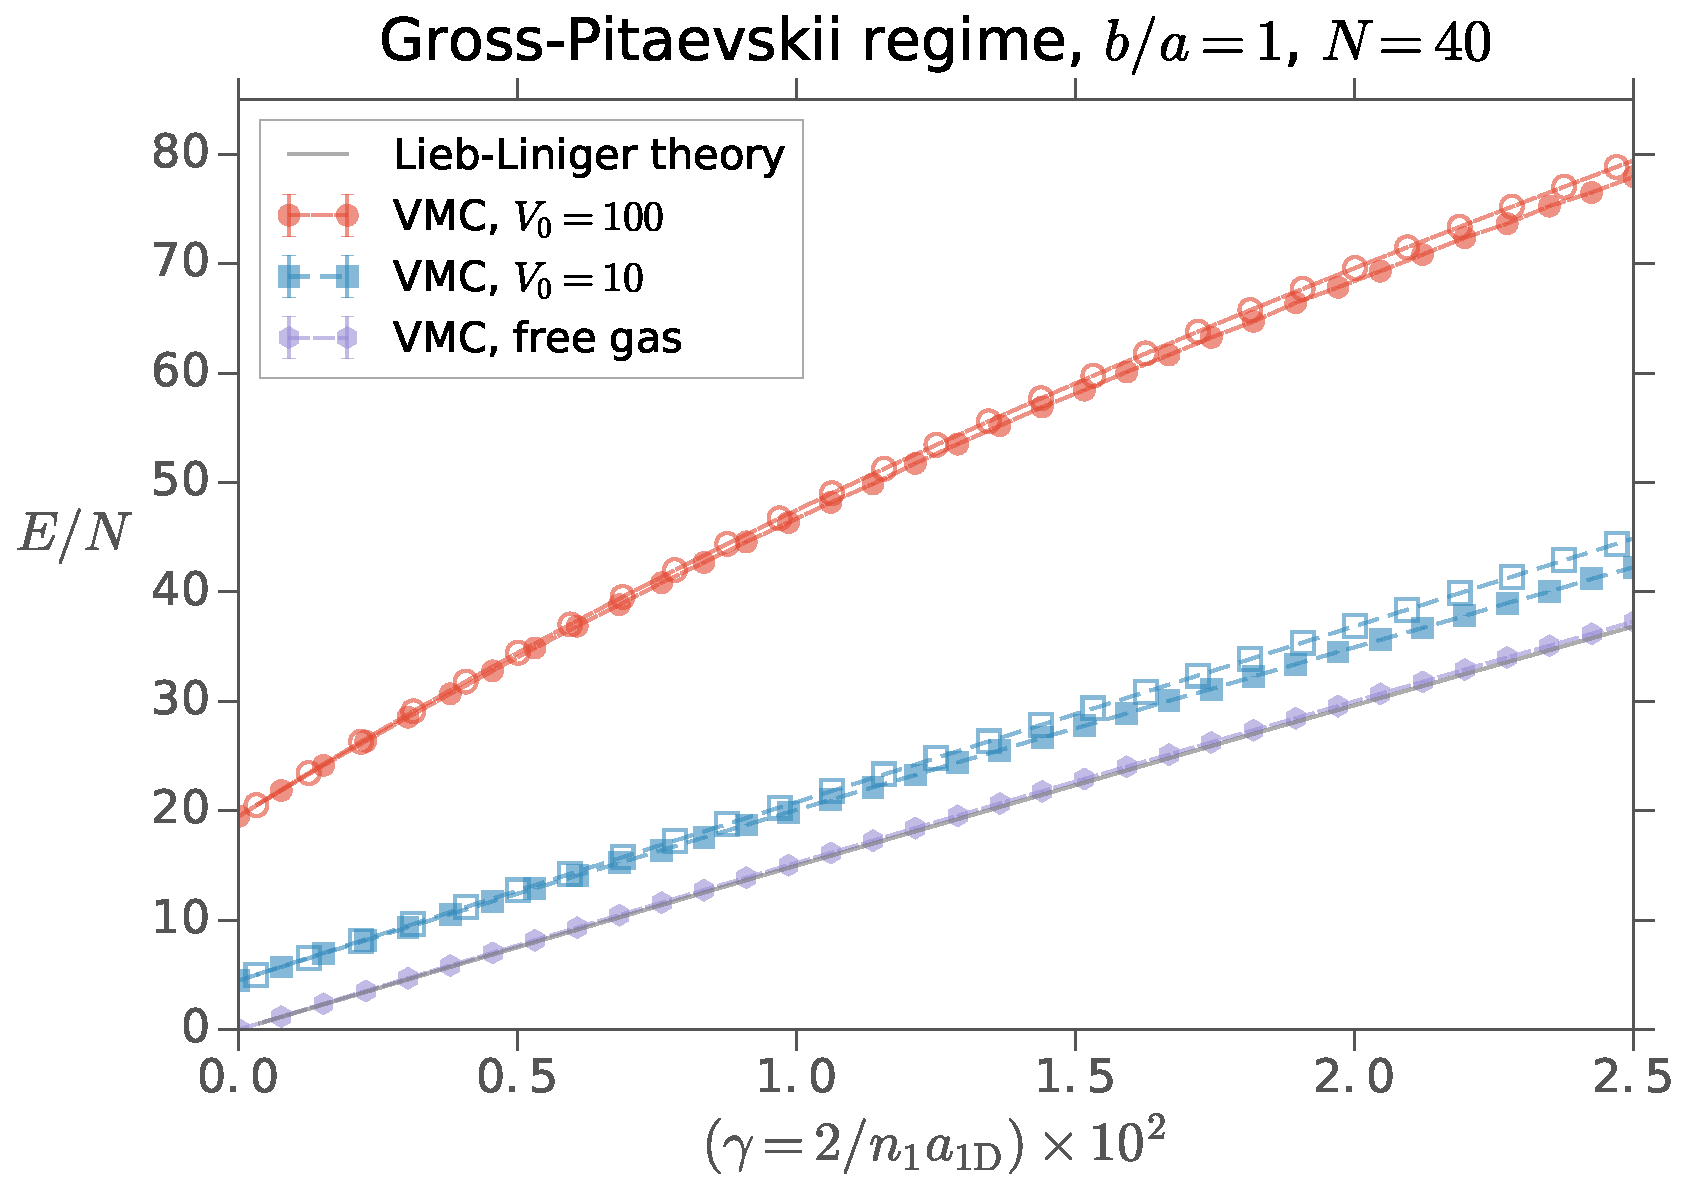
\includegraphics[width=0.75\linewidth]{./figures/phonon-gp_energy-as-gamma_rm-var_Nb-40}
  \caption{ Comparison of the energy per boson $E/N$ (in units of $\hbar^2/2m(a
      + b)^2$) as a function of $\gamma$ for different magnitudes of the external
    potential. The energies were calculated using the Lieb-Liniger theory
    \eqref{eq:lieb-liniger-energy} (solid line), VMC simulation (filled markers)
    and mean-field theory \eqref{eq:gross-pitaevskii-energy-multirods} (blank
    markers) with forty particles in the mean-field regime. }
  \label{fig:phonon-gp-energy-as-gamma-rm-var-nb-40}
\end{figure}

